\documentclass[british,titlepage]{ntnuthesis}
\raggedbottom
\usepackage{graphicx}
\usepackage{appendix}
\usepackage{lipsum}
\usepackage{array}
\usepackage{biblatex}
\usepackage{subcaption}
\usepackage{float}
\usepackage{longtable}
\usepackage{listings}
\usepackage{xcolor}
\usepackage{multirow}

\lstset{language=Python,
    basicstyle=\small\ttfamily,
    keywordstyle=\color{blue}\ttfamily,
    stringstyle=\color{red}\ttfamily,
    commentstyle=\color{green}\ttfamily,
    morecomment=[l][\color{magenta}]{\#},
    showstringspaces=false,
    breaklines=true,
    frame=tb
}


\title{Private Information Exposed by the Use of Robot Vacuum Cleaner in Smart Environments}
\shorttitle{Private Information Exposed by the Use of RVC in Smart Environments}
\author{Benjamin Andreas Ulsmåg}
\shortauthor{B. Ulsmåg}
\date{01.06.2023}
\addbibresource{thesis.bib}




% From https://www.overleaf.com/learn/latex/Glossaries

\makeglossaries % Prepare for adding glossary entries


\newglossaryentry{latex}
{
        name=latex,
        description={Is a mark up language specially suited for
scientific documents}
}

\newglossaryentry{bibliography}
{
        name=bibliography,
        plural=bibliographies,
        description={A list of the books referred to in a scholarly work,
typically printed as an appendix}
}

\newglossaryentry{maths}
{
    name=mathematics,
    description={Mathematics is what mathematicians do}
}


% --------------------
% ----- Acronyms -----
% --------------------

\newacronym{phd}{PhD}{philosophiae doctor}
\newacronym{CoPCSE}{CoPCSE@NTNU}{Community of Practice in Computer ScienceEducation at NTNU}
\newacronym{gcd}{GCD}{Greatest Common Divisor}
\newacronym{IoT}{IoT}{Internet Of Things}
\newacronym{RVC}{RVC}{Robot Vacuum Cleaner}
\newacronym{WAN}{WAN}{Wide Area Network}
\newacronym{Wi-Fi}{Wi-Fi}{Wireless Fidelity}
\newacronym{WLAN}{WLAN}{Wireless Local Area Network}
\newacronym{ISP}{ISP}{Internet Service Provider}
\newacronym{LAN}{LAN}{Local Area Network}
\newacronym{MAC}{MAC}{Media Access Control}
\newacronym{NIC}{NIC}{Network Interface Card}
\newacronym{TLS}{TLS}{Transport Layer Security}
\newacronym{VPN}{VPN}{Virtual Private Network}
\newacronym{AP}{AP}{Access Point}
\newacronym{DHCP}{DHCP}{Dynamic Host Configuration Protocol}
\newacronym{IP}{IP}{Internet Protocol}
\newacronym{OSI}{OSI}{Open Systems Interconnection}
\newacronym{SSID}{SSID}{Service Set Identifier}
\newacronym{NAT}{NAT}{Network Address Translation}
\newacronym{AWS}{AWS}{Amazon Web Services}
\newacronym{DNS}{DNS}{Domain Name System}
\newacronym{NTP}{NTP}{Network Time Protocol}
\newacronym{UDP}{UDP}{User Datagram Protocol}
\newacronym{TCP}{TCP}{Transmission Control Protocol}
\newacronym{ARP}{ARP}{Address Resolution Protocol}
\newacronym{FQDN}{FQDN}{Fully Qualified Domain Name}
\newacronym{SD}{SD}{Standard Deviation}
\newacronym{IGMP}{IGMP}{Internet Group Management Protocol} % add glossary and acronym lists before document

\begin{document}

\chapter*{Problem description}


\textbf{Title: Private Information Exposed By The Use Of Robot Vacuum Cleaners In Smart Environments}
\newline
\textbf{Student: Benjamin Andreas Ulsmåg}
\newline
\newline

The use of robot vacuum cleaner is rapidly increasing in all kinds of smart environments. Vendors are developing new smart features and APIs to allow maximum functionality and integration flexibility. Vendors develops smart phone applications, to make it easier for users to personalize their robot vacuum cleaner experience. These applications are delivered through cloud services, commando and control is communicated between smart environments and cloud services. This communication is generating network traffic in local wireless, and cabled network as well as Internet traffic. The traffic generated by the robot vacuum cleaner will reflect the actions made by users, and potentially expose user private information. An attacker can eavesdrop the network traffic in different phases in the communication. 

Smart phone application uses encrypted end-to-end communication to mitigate the risk of exposing private information. This kind of security measures are implemented by the application itself and not the network infrastructure. Information about IP-addresses, packet lengths, ports and low level protocol will still be available for attackers conduction network eavesdropping. This metadata and header information can potentially expose user private information. This thesis aims to address and determine which kind of private information that is exposed. 





\chapter*{Abstract}


\chapter*{Sammendrag}
Robotstøvsugere er blitt populære IoT enheter og er mye brukt i ulike smarte miljøer. Integrasjon med andre IoT systemer skaper flere sikkerhets og personverns utfordringer ved bruken av disse. Produsenter har utviklet applikasjoner hvor brukere kan konfigurere rengjøring og se informasjon om robotstøvsugeren etter eget ønske. Dette øker integrasjonen mellom brukernes liv og robotstøvsugeren, noe som kan eksponere mer privat informasjon. Industristandarder bruker ende-til-ende kryptering av kommunikasjon mellom applikasjonen, skytjenester og robotstøvsugere for å sikre den private informasjonen som sendes. Selv om denne informasjonen er kryptert, vil metadata i nettverkspakker fortsatt være tilgjengelig gjennom nettverksavlytningsangrep. I dette prosjektet skal vi undersøke hva slags privat informasjon som potensielt kan bli eksponert av denne dataen. En Irobot Roomba i7 ble installert i to forskjellige smarte miljøer hvor et passivt nettverksavlytningsangrep ble gjort mens ulike robotstøvsuger funksjonaliteter ble utført. Analyse av denne dataen avslørte at det var mulig å attribuere flere ulike smarte funksjonaliteter som ble utført av robotstøvsugeren, bare ved å se på Internett trafikken. Ulike signatur-baserte identifiserings algoritmer ble laget og viste en høy deteksjonsrate. Wi-Fi og Internett trafikken til robotstøvsugeren ble sammenlignet og like trafikkmønstre ble funnet, noe som gjør at deteksjonsmetodene også kan brukes for Wi-Fi trafikk. Denne oppgaven tar for seg implementasjon, konfigurasjon og analyse av nettverkstrafikk og presenterer en deteksjonsalgoritme for Irobot Roomba i7 hendelser.
\chapter*{Preface}

\tableofcontents
\listoffigures
\listoftables

\printglossary[type=\acronymtype] % Print acronyms
\printglossary                    % Print glossary

\chapter{Introduction}

 This chapter will start by briefly introduce the problem domain and motivation for this master thesis. Further it will address the research objectives, specify the scope and limitations, and summarize the scientific contribution.  
 
\section{Problem Domain}

The increase of Internet of Things (IoT) and deployment of smart environment are rapidly increasing, and are expected to increase further \cite{iotgrowth}. IoT 
devices are designed to automate and streamline users daily activities and duties. Robot vacuum cleaners, smart lighting, smart garage ports and smart door locks, are becoming a part of every smart home environment. The close integration between IoT devices and users lifes, introduces new security and privacy challenges.

Robot vacuum cleaners has become a popular smart environment device. These robots can automate floor cleaning, based on users preferences and customization \cite{roboticvacuumcleaner2021}. Integration with other IoT devices allows cleaning to be triggered based human action, which will potentially expose users behavior and routines. 

Other researchers have address security challenges on robot vacuum cleaners with penetration testing, vulnerability assessments and active network eavesdropping and interception. There has also been conducted research about passive eavesdropping in smart home environments. These have only identified action on the robot vacuum cleaners and not attributed the different events triggered. Robot vacuum cleaner event attribution, and privacy challenges associated with this, is not addressed.

\section{Research Objectives}
%what goals would you like to achieve? Please clearly define your project goals. 
%What are your research questions?

The goal of this thesis is to identify private information exposed in a smart environment, only based network traffic generated by a robot vacuum cleaner. We want to address this from an attackers perspective, and only use passive eavesdropping in the different phases of network communication. To be able to extract user private information, we want analyze and identify traffic pattern signatures. Further we want to use these signatures to attribute different events within a smart environment. The thesis' three research questions are listed below. 

\begin{enumerate}
    \item Which private information can be gathered from robot vacuum cleaner by carrying out a passive eavesdropping attack in a smart environment?
    \item How can the information exposed by the eavesdropping attack be misused by an attacker?
    \item Which security measures can be implemented to limit the exposed data and decrease the risk of misuse?
\end{enumerate}

\section{Scope and Delimitation}

The scope of this thesis is passive eavesdropping of wireless local area network (WLAN) and wide area network (WAN) traffic. No actions that will effect the traffic flow will be included. This excludes, traffic shaping, man-in-the-middle-attacks, traffic injection and similar actions. All traffic capturing and analysis, is from the perspective of an attacker. Only information that is available in the capturing files are therefor included in the thesis' analysis. This excludes decryption of traffic or knowledge about other local configurations and passwords within the environment or devices. 

Irobot Roomba i7 is the only robot vacuum cleaner considered in this thesis. This robot vacuum cleaner is connected to a separate WLAN during the entire data capturing process, allowing only cloud based communication. Local IoT communication and influence is therefore not included. Environment and network infrastructure is delimited to only basic Internet access. This exclude security implementations of firewalls, access-lists, identity management and multicast addressing, which could effect the communication. 

The complexity of eavesdropping is also not included, due to the large variety of solution in different smart environments. WAN interfaces are delivered by Internet service providers (ISP). Access to this traffic flow will not be considered, and a simulated WAN Interface is created within the local area network (LAN) of the environments. 

Analysis done through Wireshark and basic python scripting. Signature is therefore identified only by human manual analysis through these tools. This limits the analysis to only look at overall characteristics or initial traffic and Machine learning (ML).

\section{Contribution}
%Briefly describe the contribution of your work.
This thesis propose a method to extract network signatures for robot vacuum cleaners based on LAN, WLAN or WAN traffic. It includes a detection algorithm and signatures which can identify four different events, and one event collection on an Irobot Roomba i7, only based in the encrypted WAN traffic. The evaluation propose potential privacy challenges based on the results, as well as security defense mechanisms which could mitigate the impact and risk of passive eavesdropping attacks. 

\section{Thesis Structure}
%Briefly describe how the rest of your thesis is structured
This thesis is divvied into the chapters \textit{Background, Related work, Method, Analysis and Results, Evaluation, Discussion and Conclusion}. First the Background chapter will present relevant information needed to understand the topic. Related work will cover existing research on this area. Next the Method will present the different processes of selection, configuration, processing and analysis. Further the analysis and results will be presented. This is followed by an evaluation chapter to evaluate the research results. Last a discussion and conclusion chapter will compile the thesis' findings. 




\chapter{Background}

Internet connected devices is affecting human everyday life and routine more and more. The development in technology enables higher Internet speed, faster computers and huge amount of digital storage increases the usage and price for helpful devices such as air quality monitors, robot vacuum cleaners and smart door locks. All together these connected devices form smart home environment where home equipment can notify and act according to sensors or events triggered by other interconnected devices \cite{atlam2020iot}. A robot vacuum cleaner could clean when the front door is locked and all the smart light bulbs are turned off. For this to be possible the devices will have to use standard protocols and architecture to communicate with each other. 

This section will provide background information about key elements of Internet of Things (IoT), the use of these devices to enable a smart home environment. It will also introduce robot vacuum cleaners, common features, specifications and network and application architecture. At the end it will introduce techniques for capturing live traffic in wires and wireless communication. 

\section{Internet of Things}
Internet of things is a collection of interconnected physical and virtual devices communication and sharing information with each other using Internet or private networks. Autonomous devices connected to a network will be available for information sharing, event triggering and actions at any time and can act according to inputs, status or triggers from other inter connected devices \cite{atlam2020iot}. These systems takes advantage of the mass amount of devices to perform large scale information sharing, intelligence software enables the devices to become smarter and more advanced based on the information which is shared among them. The devices are heterogeneity and involved numerous different hardware components and software versions and languages \cite{atlam2020iot}.

The nature of customization of IoT devices makes the computational power and storage different, small devices like video cameras, smart door lock ect. can have limited local processors and storage and more the complexity to more centralized computational power such as could services. Data sensed by the door lock will have to be transferred to the cloud server, processed and replied with the appropriate action. This type of centralized architecture is more salable because the complexity is centralized, the challenge is therefor is ensure secure communication of the information as well as only authorized access to trigger events \cite{pavelic2018internet}. Some IoT systems need low latency and high computational capacity, smart car sensors is an example of this, self break and steering assistant will not have time to establish a secure connection to a could server, transfer information and then receive a action response. This low latency and high capacity introduce the need of edge or fog computing, the computing is therefor added closer to the IoT device if not embedded in the device itself \cite{mocrii2018iot}.  


\subsection{Smart Home}
Smart home is a commonly used to address the use of smart IoT devices to ease everyday living in consumers home, smart home devices is always on devices which collect and share information to other devices. These devices are controlled by a centralized mobile or computer which can trigger events or define event trigger environment within the smart home environment \cite{darby2018smart}. Consumers are installing various Iot devices in there home such as sensors, cameras and healthcare devices without really look into the security aspects of this. The willingness to install IoT devices is the effect of easing everyday tasks. IoT devices are designed to be easy to use in a everyday home, the use of common communication infrastructure like Wi-Fi and Bluetooth is therefore commonly used. The shared communication method by several IoT devises exposes the devices to each other, smart home devices with poor security can therefore increase the risk of other smart home devices to be attacked.

Smart home environment architecture is determined on how the smart home devices is connected and are communication with each other. The home first become smart when the different devices is communication with each other, data is analysed and actions are taken across the environment based on this data, without user interaction. Consumers role is to define the baseline of functionality which they want to use in their smart home environment \cite{mocrii2018iot}.

\subsection{Robot vacuum cleaner}

\section{Communication Protocols used by Robot Vacuum Cleaners}

All devices connected to a network need to follow standard communication protocols to be able to share information between each other. This work is the same way that humans use languages to communicate, we two persons talk different languages then they will need a converter to understand each other. In communication technology the different layers of the communication stack is divided into different communication layers. OSI reference model \cite{osimodel} is a commonly used model to describe the different layers of network communication. Each layer work separate from each other with some dependencies. The different layer is \cite{osimodel}: 
\begin{itemize}
    \item Physical layer, includes all the physical components such as, voltage, bit rate, connectors, signal transformation to the transmission medium. 
    \item Data link layer, control traffic flow and access to transmission medium on a reliable manner, point-to-point communication. 
    \item Network layer, enables traffic flow between two hosts by finding a way through the network. 
    \item Transport layer 
    \item Session layer 
    \item Presentation layer 
    \item Application layer
\end{itemize}
In the modern western society today it is common to have a mix of wires network cables delivered to you house by and ISP. This cable is often terminated in a customer edge router which delivers internet connectivity to the household. The customer edge router communicates with other devices with the use of wired communication Ethernet IEEE 802.1 or wireless by using IEEE 802.11. 

\subsection{IEEE 802.3 Ethernet}
Ethernet is a communication standard defined by the IEEE 802.3 standard \cite{802.3}. This is a mass standard in wired data link layer communication because of its adoption. The standard is also described as media access control due to the nature of ensuring link communication through wired media, this is done with standardised frames with serialized information which is captured and reads the bits according to the defined specification in \cite{802.3}. All data transmitted are collections of bytes, which includes 8 bits with the value 1 or 0. A byte can therefore hold all values between 0 to 255, this is also called a octet. A frame is divided into nine blocks: 
\begin{itemize}
    \item \textbf{Preamble field} is used to enable the receiving part of the communication to synchronise with the transmitted signal's timing.
    \item \textbf{Start frame delimiter} is a eight bit long bit sequence 10101011, to specify to the receiving system to signalize when the destination address field starts. 
    \item \textbf{Destination address} is a called a MAC address \cite{macaddress} and is described with six octets. A MAC address can be divided into two three octet parts, the first part is vendor specific and the last three octets is device specific. There is three types of destination MAC addresses defined: 
    \begin{itemize}
        \item Unicast, one source to one destination. 
        \item Multicast, one source to several destinations. Usually clients subscribe to different multicast groups if they would like to receive the data shared within this group. 
        \item Broadcast, one source to all devices on the connected data link layer network. This is used in cases where the destination address is unknown and the client flood the LAN to ensure that the frame reaches the intended destination. 
    \end{itemize}
    \item \textbf{Source address} is also a MAC address but is only used to state the initiator of traffic. 
    \item \textbf{Length/Type} specifies either the length of the embedded client data section of the frame or the client data type protocol which is the underlying protocol. This helps the receiver to determine if it needs to add padding to ensure optimal frames. 
    \item \textbf{MAC client data} includes data from the above layers in the OSI model, most commonly IP-packages. 
    \item \textbf{Padding bits} is used to make the MAC client data 
    \item \textbf{Frame check sequence}
    \item \textbf{Extension field}
\end{itemize}
\subsection{IEEE 802.11 WI-FI}

\subsection{Internet Protocol}

\section{Network traffic sniffing}





\chapter{Related Work}
This chapter introduce existing research and literature relevant for this thesis' topic. Presented work are focused around security and privacy issues, related to the topics: IoT, smart environment and robot vacuum cleaners. Further, related work on different eavesdropping attacks and possible countermeasures are described.

\section{Smart Home Security and Privacy}
The mass adoption of IoT devices in smart environments have increased the security issues within these environments. According to Alferidah and Jhanjhi \cite{Iotissues}, and Swessi and  Idoudi \cite{iotissues1} these issues are presented in all layers of the IoT systems hardware, software and communication. The nature of information sharing also introduces privacy issues in smart environments \cite{Iotissues}. Alferidah and Jhanjhi \cite{Iotissues} have created an overview of the most critical vulnerabilities and possible counter measures in an IoT environment. 

IoT smart integration enables controllers to trigger actions based on sensor data, without user interaction. Gu et al. \cite{eavsIoT} did a research on wireless Zigbee traffic mining in a smart office environment. They were able to identify and attribute 35 different events only by passively eavesdropping the wireless traffic. With further analysis they were able to expose private information about the office routines based on this traffic.  

\section{Security and Privacy Challenges of RVC}
The popularity of robot vacuum cleaners raises the concern for information security and privacy issues. Sundström and Nilsson \cite{Roborockvulnerability} looked at the security implementation and vulnerabilities on a Roborock S7. They discovered that the robot vacuum cleaner was reasonably secure. Due to ethical concerns, the cloud service security was not in scope. During the setup stage they discovered that all devices within wireless coverage of the vacuum cleaner, could add initial configuration, regardless of application support. According to Sundström and Nilsson \cite{Roborockvulnerability} the Roborock S7 was vulnerable against DHCP starvation attack from rouge devices on the same network. The authors suggested that networks used to control a Roborock should at least have basic authentication requirements, to avoid rouge devices. 
A similar research is done by Ullrich et al. \cite{Neato} where the robot vacuum cleaner was produced by Neato. In this research the authors evaluated communication and security towards the cloud service and application. They discovered that week cryptography and shared private keys among the devices resulted in a huge privacy risk. The collected data revealed personal information about the customers routines, apartment size, pets and number of residents. 

Sami et al. \cite{lindaeavesdropping} did a research on private information eavesdropping, based on laser sensor data of a robot vacuum cleaner.  This sensor data was extracted through a side-channel on the targeted robot vacuum cleaner. Through the research they were able to sense vibrations in objects like pager bags and detect words said by humans in the environment. By sensing vibrations on objects from television or music speakers they were able to identify songs and tv shows, with high precision. They suggested that manufactures have to make security implementations, limiting high precision private data to be extracted.

Nguyen \cite{robotvacuum_voulne_nguyendeep}, Kaminski et al. \cite{robotvacuum_voulne1_kaminski2016averting} and Torgilsman and Bröndum \cite{robotvacuum_voulne2_torgilsman2020ethical} all address security and privacy concerns with the deployment off different robot vacuum cleaners. They use the STRIDE threat analysis framework to identify and categorize the different vulnerabilities. They executed attacks towards the robot vacuum cleaners to expose information. In addition several security and privacy issues related to setup, LAN and cloud communication for these vacuum cleaners was discovered. All of them proposed security improvements that should be implemented by the vendors. 

\section{Eavesdropping and Event Detection}
Alyami et al. \cite{Eavs_relat_alyami2022wifi} establish a method to capture out-of-network encrypted Wi-Fi traffic, and attribute different IoT devices within a smart environment. The research had a 95 percent accuracy of identifying these devices, and in some cases also their working state. Acar et al. \cite{evas_relat_acar2020peek} also conducted a similar research on smart environments, using machine learning to identify devices and their actions. These devices used Wi-Fi, Zigbee and Bluetooth. They also suggested countermeasurements that can be implemented to defend against passive eavesdropping attribution.
Xiong et al. \cite{evas_relat_xiong2022network} proposes a network traffic flow mechanism to limit the possibilities to attribute IoT devices and events with eavesdropping. They inject dummy traffic, and delay random traffic packets to mix the network traffic sequence. This defence mechanism creates more delay and latency within the environment, and disrupted some devices and functionalities.

Trimananda et al. \cite{pingpong_trimananda2020packet} have created a tool to learn and create detection rules for IoT devices based on Wi-Fi and WAN traffic. The traffic in the research is encrypted, and they have only used packet lengths and IP address as attributes. Events are triggered through the tool, and corresponding traffic capturing is initiated. Timestamp and event capturing files are then used to train a machine learning algorithm to create event signatures. They were able to identify user behaviour within the smart home using this tool. 



\chapter*{Method}

This chapter will describe how the research is executed and which elements that is used. All Hardware, software and processes used will be described to increase the repeatability and validity of the research. The research can be divided into three, lab environment design and tests, traffic capturing and traffic analysis.

\section{}{Tests}
This section will describe the different tests and why they are relevant to the research. Attributes, settings and how the tests are performed will in detailed be described to ensure that all the tests and number of tests are performed the same way.

\section{}{Traffic capturing}
Smart home devices often generates network traffic continuous, as robot vacuum cleaners are cloud based they need to establish and keep alive a secure tunnel where commando and control can be executed. This section will describe how the captures are done and extracted to the location where the packet captures will be analysed. 

\section{}{Traffic Analysis}
To ensure that the research will produce the best contribution to the field of information security. Several different analysis tools will be used, but the main focus will be to use the best satiable machine learning algorithm for this purpose. The Traffic analysis section of this method will include the selection of there methods and, ect    

\section{Smart Home Environment}
To be able to perform passive eavesdropping on a robot vacuum cleaner there have to be set up a lab environment which is able to act similar as a normal smart home environment and allow the traffic and events to be controlled. This parts include the selection of smart home environment, it also includes the selection of devices to use such as robot vacuum cleaner, sniffing hardware and software as well as network design to allow capturing of traffic is the different phases in smart home communication. 

\subsection{Apartment}
The smart home environment will be set up in an apartment in Oslo, the whole apartment is 85m2 and the cleaning area of will be limited to the living room with 12m2. This is illustrated in figure XX. The apartment is located in the 4th floor of a brick building which have a 5th floor. This apartment is chosen because the author of this thesis lives here and it will therefore be a representative live smart home environment.

\begin{figure}[!ht]
    \centering
    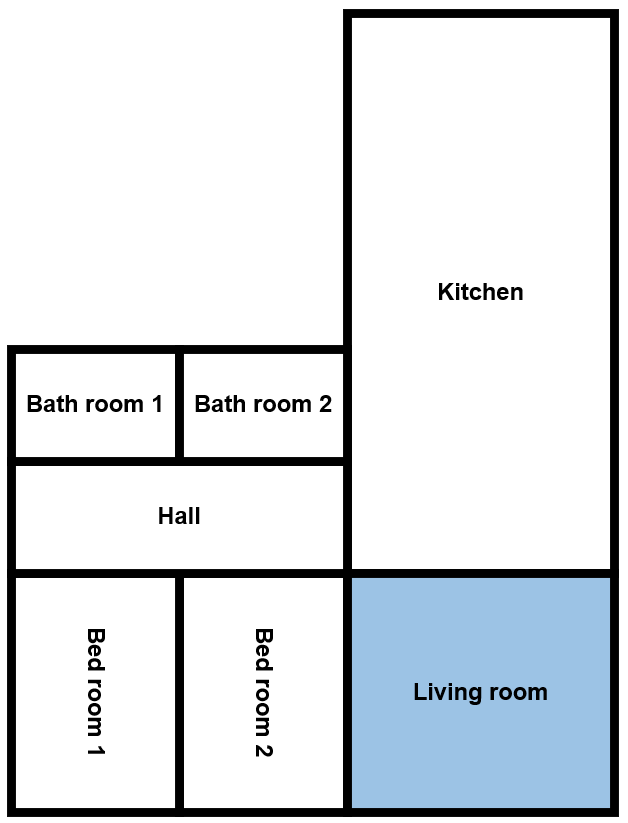
\includegraphics[width=10cm]{figures/Apartment.png}
    \caption{Network High Level Design}
    \label{fig:HLD}
\end{figure}

 The living room is 3,30m x 3,64m and aprox 12 m2. and includes furniture as shown in the figure XX. 

\begin{figure}[!ht]
    \centering
    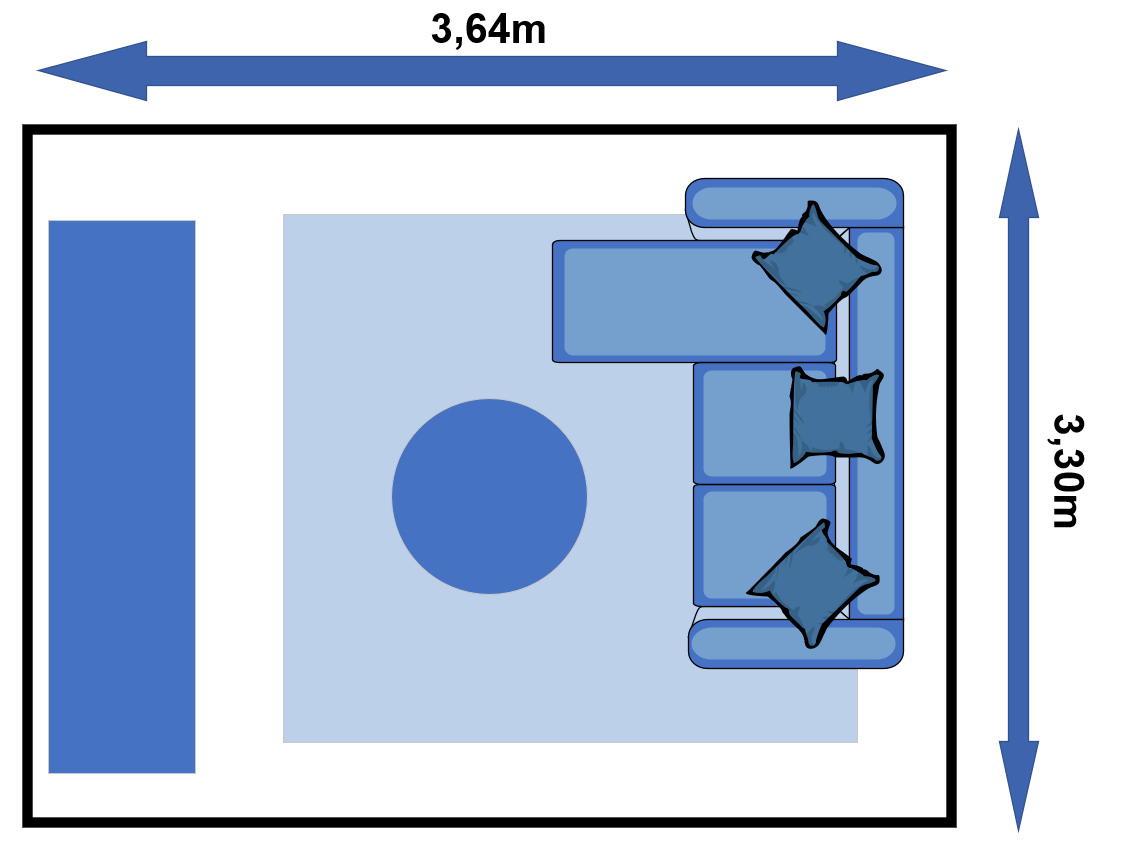
\includegraphics[width=10cm]{figures/Living room.png}
    \caption{Network High Level Design}
    \label{fig:HLD}
\end{figure}

\subsection{Robot vacuum cleaner}
The robot vacuum cleaner is the main device in this research. To select the best suited vacuum cleaner we did a selection survey which based on the requirements we had about different smart home features, price, norwegian distributor and popularity. The survey selected resulted in Irobot roomba 7i as the best option. The selection process and secifications for Irobot roomba i7 is described in subsections below.

\subsubsection{Robot vacuum selection}
Because of limited resources and time, the selection of equipment needs to be done before acquiring anything. The vacuum will need several smart home features so that the different features can be identified in the network traffic analysis. The purpose of this research is to identify how much private information which can be gathered as well as how complex these types of sniffing attack will have to be. Selecting a vacuum cleaner with more smart home features will potentially reveal more sensitive private information.

    \paragraph{Communication network protocols:} IoT devices can use several different network protocols and technology to communicate with other devices. We distinguish between Datalink layer (layer 2), Network layer (layer 3), session layer (layer 4) and Application layer (layer 5). Each of these layers can reveal different information about the session, devices and data which is sent. The Data Link Layer protocol IEEE 802.11 (Wi-Fi) it is the most widespread infrastructure in smart homes \cite{robotsel1}. Wi-fi will therefore be the preferred data link layer protocol, this to ensure the most relevant result \cite{robotsel2}\cite{robotsel3}. The selection of IEEE 802.11 will result in more common Internet routing protocols which supports the principle.

    \paragraph{App features:} To enable the best user experience possible more and more IoT devices comes with dedicated application for command, control, statistics, and integration. Such applications add new smart home features to devices which often result in more data transfers between the device and the cartelized controller. The application architecture is dependent on the vendor, but a common design is a client-server architecture, where both the vacuum cleaner and mobile application is acting as clients \cite{robotsel4}. This may include sensitive private information transferred between the devices. \cite{robotsel7}

    \paragraph{Navigation:}A robot vacuum cleaner will have to navigate around the smart home to be able to clean sufficiently. This navigation is handled differently, form the basic to more advanced navigation. Some of the more advances navigation systems uses laser or camera to navigate and map the environment. \cite{robotsel5} \cite{robotsel6} This type of mapping could generate some interesting information for the research. 

\paragraph{}Open-source information, tests sites and YouTube videos are used to gather information to base the selection on. To limit the number of relevant robot vacuum cleaner vendors I used open source review sites to determine which vendors that had the highest ranking robots. Next, I used Google Play and the available statistics to see how many downloads and rating the different vendor specific application had. Based on the results from these findings I filtered the vendor models based on app features and navigation described in the introduction, the best suited robot vacuums per vendor is then compared to each other to finally select one. Prices are gathered from the comparison website prisjakt.no\cite{prisjakt.no}. 

 From opensource test sites there was two robot vacuum vendors which did good, Irobot and Roborock, these are therefore the main vendors to be considered. As reference to another popular vendor Xiaomi is also included in the survey.\cite{robotsel11}\cite{robotsel12}\cite{robotsel13}

\paragraph{Selection:} \cite{robotsel11}\cite{robotsel12}\cite{robotsel13} is used as vendor comparison review sites, these were selected because they were some of the top results on my google with the search string “Robot vacuum cleaner test”. The vendor on top ten selection \cite{robotsel11} is listed in tabel XX, \cite{robotsel12} listed in tabel XX and \cite{robotsel13} listed in tabel XX. 

\begin{table}[]
\begin{tabular}{|l|c|}
\hline
Vendor   & Number on top ten \\ \hline
Roborock & 3                 \\ \hline
Irobot   & 3                 \\ \hline
ILife    & 2                 \\ \hline
Wyze     & 1                 \\ \hline
Neato    & 1                 \\ \hline
\end{tabular}
\end{table}


\begin{table}[]
\begin{tabular}{|c|c|}
\hline
Vendor    & Number on top ten \\ \hline
Ecovacs   & 2                 \\ \hline
Irobot    & 2                 \\ \hline
Roborock  & 2                 \\ \hline
Shark     & 1                 \\ \hline
Eufy      & 1                 \\ \hline
ILife     & 1                 \\ \hline
Proscenic & 1                 \\ \hline
\end{tabular}
\end{table}

\begin{table}[]
\begin{tabular}{|c|c|}
\hline
Vendor   & Number on top ten \\ \hline
Irobot   & 2                 \\ \hline
Roborock & 2                 \\ \hline
Neatsvor & 3                 \\ \hline
Ecovacs  & 1                 \\ \hline
Neato    & 1                 \\ \hline
Kyvol    & 1                 \\ \hline
\end{tabular}
\end{table}

\begin{table}[]
\begin{tabular}{|c|c|}
\hline
Vendor    & Number on top ten \\ \hline
Irobot    & 7                 \\ \hline
Roborock  & 7                 \\ \hline
Neatsvor  & 3                 \\ \hline
Ecovacs   & 3                 \\ \hline
ILife     & 3                 \\ \hline
Neato     & 2                 \\ \hline
Proscenic & 1                 \\ \hline
Wyze      & 1                 \\ \hline
Shark     & 1                 \\ \hline
Eufy      & 1                 \\ \hline
Kyvol     & 1                 \\ \hline
\end{tabular}
\end{table}

To get a briefly overview of the popularity of the different robot vacuum cleaners we can use the number of downloads of the different applications. This information is available in Google play with overall user rating, application rating is also available in Apples App Store. 

\begin{table}[]
\begin{tabular}{|c|c|c|}
\hline
Application & Google play download & App rating 0-5 \\ \hline
Irobot      & 5 million+           & 4,0            \\ \hline
Roborock    & 1 million +          & 4,6            \\ \hline
Xiaomi      & 10 million +         & 4,3            \\ \hline
Ecovacs     & 1 million +          & 2,5            \\ \hline
Shark       & 1 million +          & 3,3            \\ \hline
Eufy        & 1 million +          & 4,6            \\ \hline
ILife       & 10 thousand +        & 2,2            \\ \hline
Wyze        & 1 million +          & 4,0            \\ \hline
Proscentic  & 100 thousand +       & 2,0            \\ \hline
\end{tabular}
\end{table}

As we can see the most downloaded applications in google play is “Irobot” and “Xiaomi”, the difference between these two applications is that Irobot is a pure vacuum cleaner application and Xiaomi is a smart home application where you can connect other IoT devices and control your integrated smart home.  
Satisfaction based on rating is also divided between the different application, applications with the rating above 3.9 is: Irobot, Roborock, Xiamoi, Eufy and Wyze. 

\paragraph{Discussion} Based on the open-source top ten site review the results showed that Irobot and Roborock was the overall best vendors on the marked. These are therefore the most relevant vendors to compare to find the most suited vacuum cleaner to our project. This assumption is also supported when it comes to the results from Google play statistics, there we can see that both Irobot and Roborock is among the highest rated and downloaded applications. These two results make us confident that a vacuum cleaner from one of these vendors will give us a popular and well used vacuum cleaner which makes the research results more relevant. 
Xiaomi is the most downloaded application in Google play with more than 10 million downloads, in difference with the applications from iRobot and Roborock the application is designed to handle an entire smart home and not just vacuum cleaners. As Xiaomi has a lot of other IoT devices on the marked this could cause more downloads which is not directly connected to the use of their vacuum cleaners. Is was also not mentioned in any of the top ten review sites which we used and is therefore not the right fit for this research. If the purpose was to analyse an entire smart home, it could be more relevant due to the integration features in the smart home application. 
Most suitable vendor vacuum: 
Irobot Roomba I7 is the most suitable model from Irobot in this research project. This is the model which includes all the smart features included through the app without extra cost associated with extra cleaning features. Compared to the I6 model I has newer hardware and support for minimal cost. \cite{robotsel9}

\paragraph{Conclution} Both iRobot Roomba i7 and Roborock has a lot of the same features which is must have on a robot vacuum cleaner, as well as they are in the same price range. The advantage of 5 million downloads vs Roborock’s 1 million indicated that the iRobot vacuum cleaners are more used combined with smart home features. The iRobot also has seasonal and pet detection and can make suggestions on the cleaning patters, this ability to identify user behaviour could create a lot of sensitive private information about it’s roommates. iRobot Roomba i7 will therefore be the most suitable robot vacuum cleaner for this research




\subsubsection{Network design}
To represent the general smart home in common homes the research used the existing network infrastructure in the apartment and added some components to be able to better isolate the traffic from the robot vacuum cleaner. The different elements are show in figre \ref{fig:HLD}, further each device will be described. 

\begin{figure}[!ht]
    \centering
    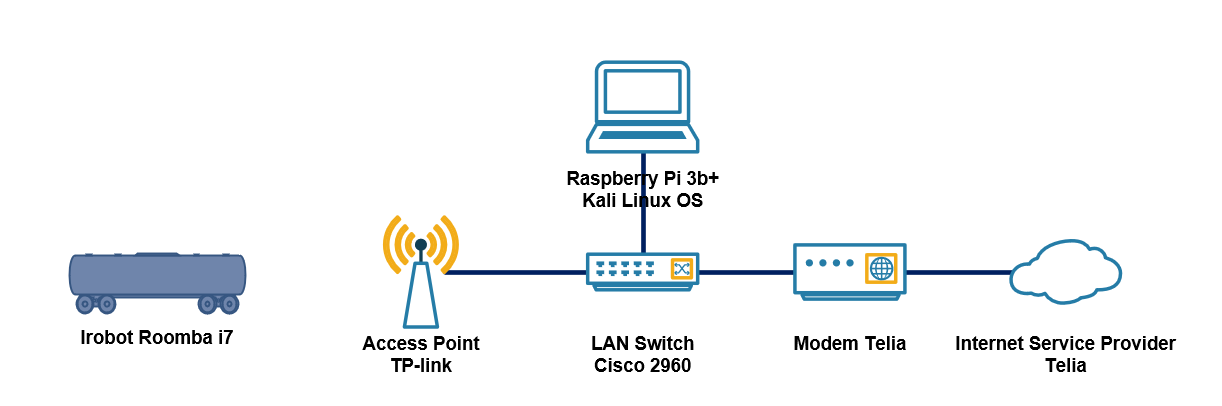
\includegraphics[width=10cm]{figures/HLD.png}
    \caption{Network High Level Design}
    \label{fig:HLD}
\end{figure}

\begin{itemize}
    \item \textbf{Device:} Raspberry Pi 3b+
    \item \textbf{Software:} Kali ARM \cite{kalidownload}, updated 27.09.2022
    \item \textbf{Configuration:}
    \begin{enumerate}
        \item Image downloaded to an external computer and written to the micro SD-card with the application balenaEtcher \cite{balenaetcherdownload}.
        \item Patching done 19.12.2022 with the command "sudo apt update \&\& sudo apt upgrade"
    \end{enumerate}
    \item \textbf{Connected items:}
    \begin{enumerate}
        \item Micro SD card \cite{microsdcard}
        \item TL-WN722N USB WiFi Adapter \cite{tp-link}
    \end{enumerate}
\end{itemize}

\section{Test cases}
Each test Case consists of a detailed test description, which enables the tests and results to be reproduced as identical as possible. It will also state how many times the test was done during the research. The standby traffic test is performed over 14 consecutive days, and all other tests are done 20 times. The number of days and tests are decided based on the available time frame for this master thesis. Equipment selection process, design and configuration process and test phase is time consuming and 20 is therefore chosen as the overall test number. 

\subsection{Baseline-traffic}
Baseline test have the function to represent the traffic flow generated by the robot vacuum cleaner installed in the smart home environment with out any event triggering. For this test the robot vacuum cleaner is installed in the chosen smart home environment described in "smart home environment chapter". Before the test was conducted the robot was operational for more then 60 days, and more then 10 cleaning jobs done. This to ensure that is is in operational mode.

\begin{itemize}
    \item \textbf{Description:} Conduct packet sniffing for both wireless and cabled traffic generated over a number consecutive days. Capture data is stored in two separate files. The Robot vacuum cleaner is connected to power and Internet the entire time period.
    \item \textbf{Number of tests:} 14 consecutive days
\end{itemize}

\subsection{Triggered cleaning}
Triggered cleaning is an event started trough the IRobot application with the use of "start cleaning". The test is done when the mobile application receives a notification that the cleaning is done. If the robot vacuum need to return to base to recharge, empty bin or get stuck something in the brushes, actions will be done to enable the robot to continue cleaning. 
\begin{itemize}
    \item \textbf{Description:} Start cleaning through the Irobot application, with the use of start cleaning. Capture is started 10 minutes before cleaning is scheduled and stopped 30 minutes after the cleaning is finished. 
    \item \textbf{Number of tests:} 20
\end{itemize}

\subsection{Empty bin} The bin needs to be removed from the vacuum cleaner to be emptied. This will make the vacuum cleaner in a state where is cannot start cleaning, and the application will display information about the situation. 

\begin{itemize}
    \item \textbf{Description:}Start packet capturing 5 minutes before the bin is removed. Remove the bin, wait 5 minutes and then insert the bin once more. Stop capturing 5 minutes after the bin is inserted
    \item \textbf{Number of tests:}20
\end{itemize}

\subsection{Open mobile application}
Mobile application will be able to access information about the robot vacuum cleaner. This might generate pull requests from the Irobot cloud towards the vacuum cleaner to get the needed information to display. If the user changes attribute in the application this needs to be communicated with the vacuum cleaner. 
\begin{itemize}
    \item \textbf{Description:} Start packet capturing 5 minutes before opening the application on the smart phone. Open the application, change a "room name" and one "room separation line", then wait until the application have been open for 5 minutes, then close the application. Stop packet capturing after additionally 5 minutes. 
    \item \textbf{Number of tests:}20
\end{itemize}



\section{Methods in relates work}
Through some one the papers review in the related work section they used to capture live traffic from the smart devices.In this section the different methods in \cite{lindaeavesdropping} \cite{eavsIoT} \cite{Neato}, will be discussed and elements that could be used in this research will be identified and justified. 


\begin{itemize}
    \item \textbf{Description:}
    \item \textbf{Number of tests:}20
\end{itemize}
\chapter{Analysis and Results}
\label{cap:AnalysisandResults}

This chapter presents the analysis and results of standby traffic and event captures. First the standby traffic is analysed to identify traffic irrelevant to the event objectives triggered. This is followed by a section for each event including analysis and results of overall event characteristics, protocol detection and packet sequences resulting in a signature detection algorithm. \gls{WAN} traffic is compared with the corresponding \gls{WLAN} traffic to identify if these signatures are applicable in both transmissions domains. 

\section{Standby Traffic}
This section presents the analysis of the captured \textit{Standby traffic} to identify traffic patterns or protocols to exclude in further event analysis. First an analysis of the relevance of the different identified protocols is conducted. All occurring traffic patterns within the standby event can be found in the event captures as well, but are irrelevant for the actual event triggering.

The standby event capturing was conducted from 8th of January to 22th of January 2023 in \textbf{Oslo} environment. During this time period there was no physical or application interacting with the Irobot Roomba, all traffic captured was therefore generated by the Irobot Roomba or the connected Irobot cloud service. This traffic is not created by any human interaction and not exposing any private information. Beforehand, the Irobot Roomba had been installed and operated for one month, ensuring that it was in an operating and not installation state. Smart home map, room dividers and customized cleaning jobs were configured. 

Wireshark protocol hierarchy analysis tool was used to display protocol statistics and Table \ref{tab:ProtocolStatistics} presents the protocols and distribution of them. Approximately 50\% of the captured traffic was identified as \gls{UDP} traffic, this is mainly \gls{DNS} but also some NTP and \gls{DHCP} traffic. Another 26.2\% was \gls{TCP} where the majority of the captured traffic is \gls{TLS} which is used by the Irobot Roomba to ensure end-to-end encryption with the cloud server. The last protocol identified was \gls{ARP} representing 24,6\% of the standby traffic. 


\begin{table}[H]
\centering
\caption{Protocol hierarchy and statistics in standby traffic capture }
\label{tab:ProtocolStatistics}
\begin{tabular}{|c|c|c|c|}
\hline
\multicolumn{1}{|c|}{\textbf{Transport protocol}} & \textbf{Percentage}     & \textbf{Service protocol} & \textbf{Percentage} \\ \hline
\multirow{3}*{UDP}                              & \multirow{3}*{49,2} & \gls{DHCP}    & 0,1            \\ \cline{3-4} 
                                                  &                         & \gls{DNS}                       & 48,6                \\ \cline{3-4} 
                                                  &                         & NTP                       & 0,4                 \\ \hline
TCP                                               & 26,2                    & NA                        & NA                  \\ \hline
ARP                                               & 24,6                    & NA                        & NA                  \\ \hline
\end{tabular}
\end{table}

The network architecture in \textbf{Oslo} and \textbf{Drammen} creates a single broadcast domain between the AP, capturing platform and the \gls{ISP} router. As devices only use physical layer \gls{MAC} addresses to communicate on the \gls{LAN} they need \gls{ARP} to create an \gls{IP} to \gls{MAC} forwarding table. \gls{ARP} traffic is therefore broadcasted between these devices requesting updates on \gls{IP} to \gls{MAC} information. The captured \gls{ARP} traffic is not generated by the vacuum cleaner in another broadcast domain and is added as a part of the basefilter with the logical expression \textit{!arp}.

The \gls{ISP} modem is by default configured as the local \gls{DHCP} server allocating, reserving and leasing \gls{IP} addresses to devices connected to the \gls{LAN}. To ease the detection of the simulated \gls{WAN} traffic a \gls{DHCP} reservation was configured on the \gls{ISP} routers for the AP's \gls{LAN} \gls{MAC} address in both \textbf{Oslo} and \textbf{Drammen}. This kept the simulated \gls{WAN} address from changing during capturing and potentially lose traffic. \gls{DHCP} traffic was still needed to be exchanged between the \gls{AP} and the \gls{ISP} modems requesting and verifying that the reserved \gls{DHCP} leases still were active during capturing. \gls{DHCP} traffic in the \gls{LAN} capture is therefore only generated by the \gls{AP} and the \gls{ISP} modem and was added to the basefilter with the logical expression \textit{!dhcp}.

The most dominant protocol in the standby capture was \gls{DNS} with 49.2\% of the packets. 98.3\% of these \gls{DNS} packets were requests and responses for the \gls{DNS} A record for \gls{FQDN} \textit{a.root-servers.net}, this traffic flow is shown through Wireshark in Figure \ref{fig:dns_a-root}. This is one of the \gls{DNS} top level domain servers in the \gls{DNS} hierarchy and will only point to top level domain server such as .com, .org and .no. By analyzing the management console of the AP, it was observed that the \gls{AP} requested the \gls{DNS} record for \textit{a.root-servers.net} to determine if it had Internet connectivity or not. A successful response will indicate Internet connectivity. These \gls{DNS} packets are therefore irrelevant in the analysis of Irobot Roomba traffic and are specifically excluded in a Wireshark filter for further \gls{DNS} analysis with the following filter  \textit{((dns) \&\& !(frame.len ==78 or frame.len ==94))}. Frame lengths of 78 and 94 bytes are used to identify the \gls{DNS} request and response in Figure  \ref{fig:dns_a-root}

\begin{figure}[H]
    \centering
    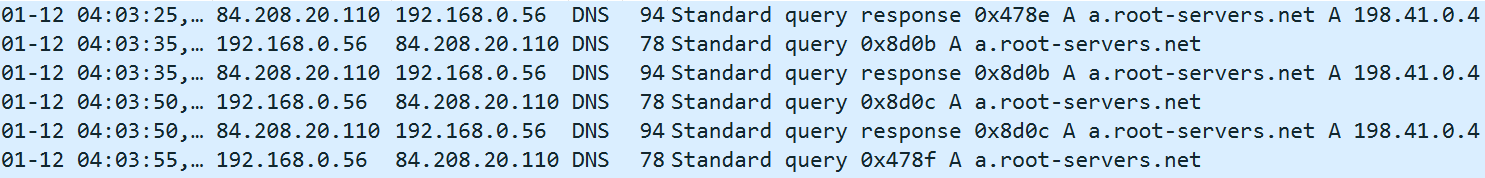
\includegraphics[width=\textwidth]{figures/DNS_a-root.png}
    \caption{Reoccurring DNS traffic associated with a.root-server.net}
    \label{fig:dns_a-root}
\end{figure}

When the filter was applied only 174 \gls{DNS} packets were left. In the remaining \gls{DNS} traffic it was observed several \gls{DNS} requests and responses generated by the \gls{AP} towards the TP-Link cloud services, these \gls{FQDN}s are listed below and shown in Figure \ref{fig:tp-link_fqdn}. 

\begin{itemize}
    \item n-devs-gw.tplinkcloud.com
    \item n-deventry-gw.tplinkcloud.com
\end{itemize}

\begin{figure}[H]
    \centering
    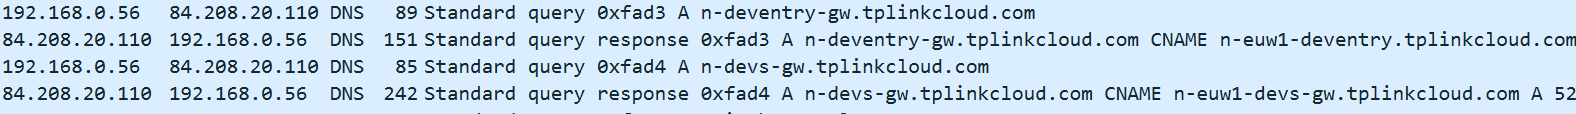
\includegraphics[width=\textwidth]{figures/DNS-tp-link.png}
    \caption{DNS traffic generated by the \gls{AP} towards TP-Link cloud services}
    \label{fig:tp-link_fqdn}
\end{figure}

These \gls{DNS} packets are excluded because they are related to the \gls{AP} and not the \gls{RVC}. After exclusion only four different \gls{FQDN} requests generated by the Irobot Roomba were displayed. Three of the \gls{FQDN} are towards the \textit{.irobot} domain and the last one is a part of .\textit{amazoneaws}. Amazone \gls{AWS} is a large provider of cloud services and bought Irobot cooperation in 2022 \cite{irobot2023_amazone} and is therefore using Amazone \gls{AWS} for their cloud services. These \gls{FQDN}s are listed below. 

\begin{itemize}
    \item 0.irobot.pool.ntp.org
    \item disc-prod.iot.irobotapi.com
    \item unauth1.prod.iot.irobotapi.com
    \item a2uowfjvhio0fa.iot.us-east-1.amazonaws.com
\end{itemize}

All \gls{DNS} traffic generated by the Irobot Roomba are occurring regularly throughout the entire standby traffic time period, this is presented in Figure \ref{fig:dns_irobot_graph}. Irobot's public NTP server \textit{0.irobot.pool.ntp.org} is requested each 12th hour,  in the project's standby traffic this is at 03:36 and 15:36. This is used to synchronize the local clock on the Irobot Roomba to a global time zone, allowing all actions or smart features using time to operate correct. \textit{disc-prod.iot.irobotapi.com}, \textit{unauth1.prod.iot.irobotapi.com} and \textit{a2uowfjvhio0fa.iot.us-east-1.amazonaws.com} are all requested once a day at the same time. The function of these requests are not identified, but when trying to access the \gls{FQDN}s through Google Chrome it prompts \textit{"Missing Authentication Token"}, based on the naming convention of the \gls{FQDN}s it is easy to believe that they are used for re-authentication of the Irobot Roomba. 

\begin{figure}[H]
    \centering
    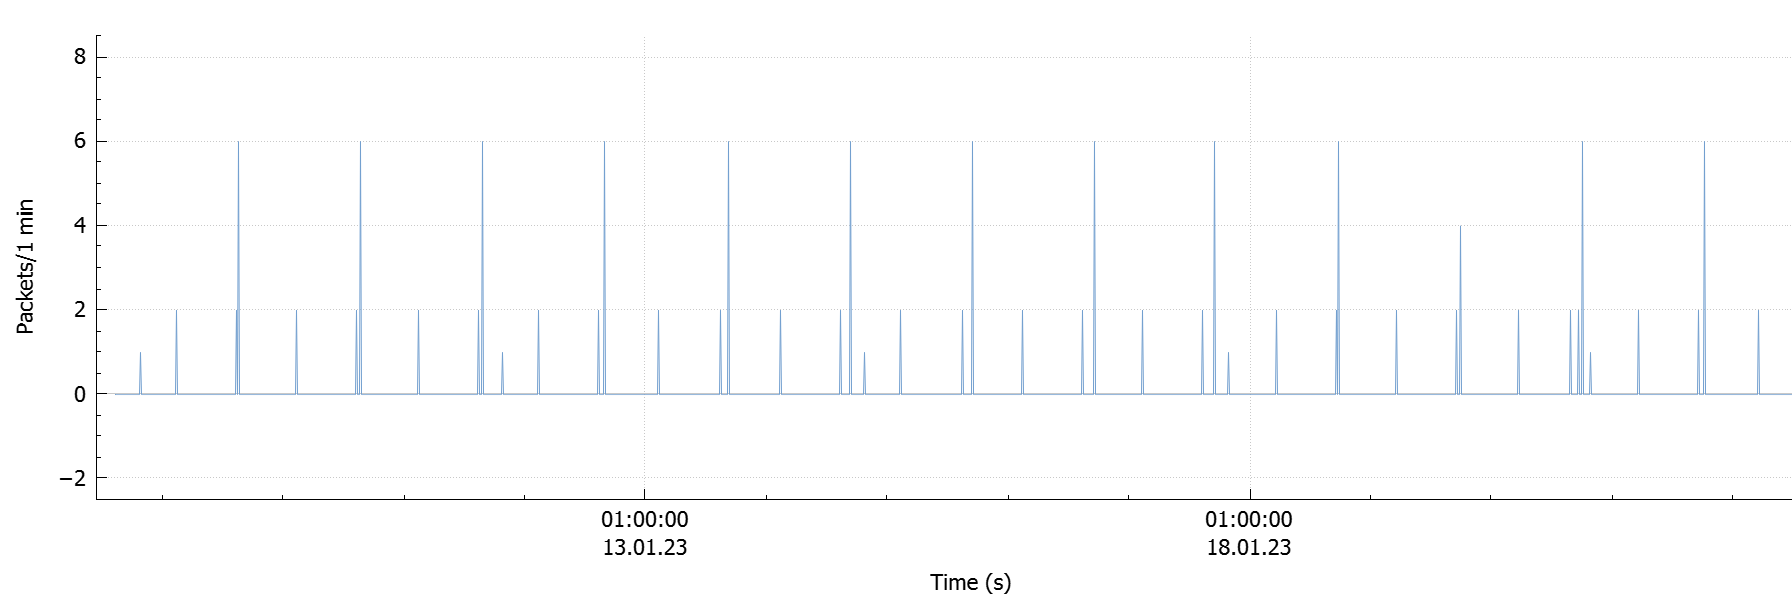
\includegraphics[width=\textwidth]{figures/DNS_irobot_graph.png}
    \caption{Irobot's reoccurring \gls{DNS} traffic presented in graphical view}
    \label{fig:dns_irobot_graph}
\end{figure}

The \gls{DNS} observations identifies that the Irobot Roomba is depending on \gls{DNS} to be able to access Irobot's cloud services. This protocol is a potential indication of cloud functionality, used or access by the Irobot Roomba and is included in further analysis of events. \gls{DNS} request for \textit{a.root-servers.net} had to be excluded due to the large amount. All Irobot generated \gls{DNS} requests had a packet size larger then 78 bytes as shown in Figure \ref{fig:dns_a-root} and all responses were larger then the response for \textit{a.root-server.net}. As the \gls{DNS} response is the most interesting part of the communication it is safe to exclude all \gls{DNS} packets smaller then 94 bytes without missing any \gls{DNS} responses towards the Irobot domains. 

\gls{NTP} server-client sessions are identified every 30 minutes generating a large volume of \gls{NTP} traffic. When observing \gls{DNS} requests to Irobot's public \gls{NTP} service \textit{0.irobot.pool.ntp.org} and \gls{NTP} traffic in Wireshark it is possible to identify that the Irobot Roomba is changing the corresponding \gls{NTP} server every time the \gls{DNS} response is received, this is shown in Figure \ref{fig:irobot_ntp_dns}. Since the \gls{NTP} traffic is continuous it is not related to events triggered, and can be excluded from further analysis by adding the logical expression \textit{!ntp} to the basefilter.

\begin{figure}[H]
    \centering
    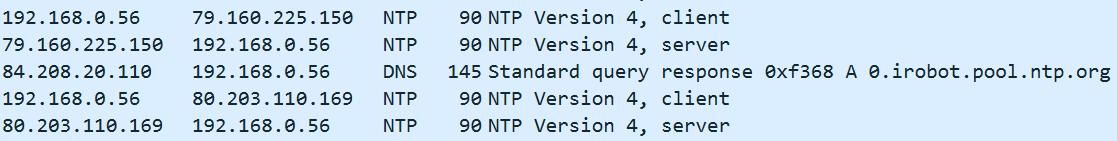
\includegraphics[width=\textwidth]{figures/NTP-irobot.png}
    \caption{Irobot NTP client-server traffic}
    \label{fig:irobot_ntp_dns}
\end{figure}

\gls{TCP} traffic was analyzed in the same manner as the network service protocols \gls{ARP}, DHCP, \gls{DNS} and \gls{NTP}. Remaining \gls{TCP} traffic is then displayed in Wireshark and is shown in Figure \ref{fig:tcp_keep-alive}. Wireshark's protocol hierarchy statistic tools identified that 64.4\% of the remaining \gls{TCP} packets uses \gls{TLS} to secure the connection, this aligns with the observations in Figure \ref{fig:tcp_keep-alive} where the reoccurring \gls{TCP} pattern consists of two \gls{TLS} packets including payload information and one empty \gls{TCP} acknowledge packet confirming that the last packet was received. Continuous \gls{TCP} traffic is generated to keep the \gls{TCP} connection between the Irobot Roomba and the cloud service open as \gls{TCP} has a timeout value on all session. The majority of smart environments are installed behind \gls{NAT} and the \gls{TCP} session must therefore be initiated from the distributed \gls{IoT} devices.  Keep-alive traffic includes the least amount of data needed to keep the connection alive or continuously updated. All event specific packets are therefore larger than 97 bytes.  This filter is combined with the \gls{DNS} packet length filter and is applied with the logical expression \textit{(frame.len > 97)} excluding all packets less than 97 bytes.

\begin{figure}[H]
    \centering
    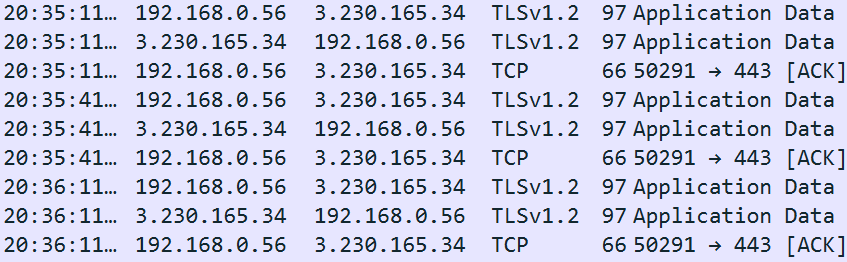
\includegraphics[width=\textwidth]{figures/tcp_keep-alive.png}
    \caption{Roccuring \gls{TCP} traffic from the standby capturing displayed in Wireshark}
    \label{fig:tcp_keep-alive}
\end{figure}

Commando and control traffic from the Irobot's cloud services is generated from the same corresponding host as the TCP-keep-alive traffic. To identify the \gls{FQDN} used in this session establishment, a combined filter with \gls{DNS} and \gls{TCP} is applied, as shown Figure \ref{fig:tcp_keep-change_dns}. As presented the Irobot Roomba terminated the \gls{TCP}-keep-alive session right before a \gls{DNS} request is sent for \textit{a2uowfjvhio0fa.iot.us-east-1.amazonaws.com}, and a new session is established with one of the \gls{IP} addresses in the \gls{DNS} response. After the establishment of the new session there is uploaded data to the new host, probably synchronising and updating current status on the Irobot Roomba.

An attacker will have to eavesdrop traffic for less than 24 hours to be able to identify which \gls{TCP} session belongs to the Irobot Roomba. In a large scale eavesdropping attack attackers can trigger actions based on identification of this \gls{DNS} response, knowing that a Irobot vacuum cleaner is establishing a new session with one of the responded \gls{IP} addresses. 


\begin{figure}[H]
    \centering
    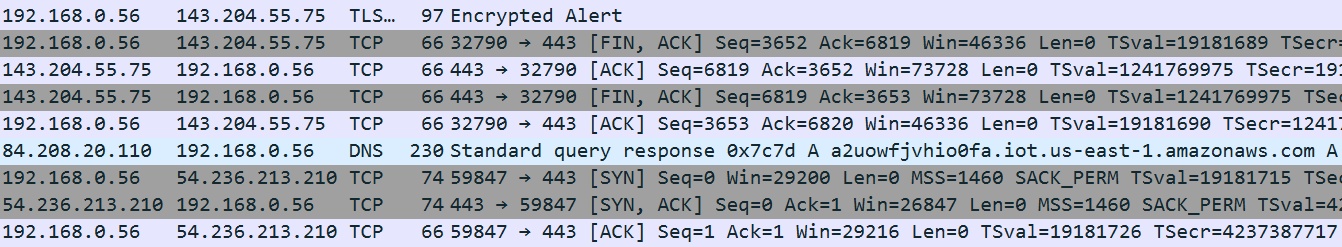
\includegraphics[width=\textwidth]{figures/wireshark_irobot_cloud_dns.png}
    \caption{Identification of Irobot commando and control traffic displayed in Wireshark}
    \label{fig:tcp_keep-change_dns}
\end{figure}

A base filter is created based on the observations described earlier in this section to exclude irrelevant standby traffic from further analysis of events. \gls{DNS} online verification generated by the \gls{AP} and \gls{TCP}-keep-alive traffic is excluded with the same logical expression excluding all packets smaller then 98 bytes, \textit{(frame.len > 97)}. This leaves the \gls{DNS} responses to other Irobot cloud services which can be used for service attribution. \gls{ARP}, \gls{DHCP} and \gls{NTP} are excluded due to functionality. The base filter created and used in following analysis of event captures are presented below. When this filter was applied to the \textit{Standby traffic} capture the total number of packets was reduced from 5,052,284 to 4,010 displaying only 0.8\% of the captured traffic.

\begin{itemize}
    \item \textit{(!ntp \&\& !dhcp \&\& !arp \&\& frame.len > 97)}
\end{itemize}


\section{General Event Analysis}

 This section introduces the general capturing process conducted in both \textbf{Oslo} and \textbf{Drammen} environment. Considerations and observations used during the event triggering process are also presented. 

 Capturing is started on the Raspberry PI for both \gls{WLAN} and \gls{LAN}, filters used on \gls{WLAN} captures are the same in both environments due to static \gls{WLAN} \gls{MAC} address for the Irobot Roomba. This \gls{MAC} address is found through the Irobot home application. However the simulated \gls{WAN} address is different, in Oslo environment is was 192.168.0.56 and in Drammen is was 192.168.0.91, the reason for this was that the \gls{IP} address reserved in Oslo was already in use within the Drammen \gls{LAN}. Tshark commands for \gls{WLAN}, Oslo \gls{LAN} and Drammen \gls{LAN} is listed below. 

 \begin{itemize}
     \item \gls{WLAN}: \textit{sudo tshark -i wlan1 -f 'eth.host 50:6F:0C:2F:EB:A2' -w 'output.pcap'}
     \item Oslo: \textit{sudo tshark -i eth0 -f 'ip.host "192.168.0.51' -w 'output.pcap'}
     \item Drammen: \textit{sudo tshark -i eth0 -f 'ip.host "192.168.0.91' -w 'output.pcap'}
 \end{itemize}

 The initiated capture was continuous running in both environments during the entire event triggering, since the output files never exceeded 500MB. During the capturing all event objectives were triggered 10 times per environment, resulting in 20 captures per event in total. All cleaning events were triggered and identified as finished when the smart home application prompted a "finished cleaning" notification. Both start and end time for all events was noted and used in the event file extraction. 

 When all event triggering was conducted, the capturing was stopped and the environment capturing file, including all triggered events, were extracted to another computer via WinSCP file transfer application. The pcap files were opened in Wireshark and a time filter was applied to extract individual files for each of the different triggered events, resulting in 20 different files for each of the event objectives. Timefilter syntax and example is presented below. 
 \begin{itemize}
     \item \textit{(frame.time >= "Month day, year hh:mm:ss") \&\& (frame.time <= "Month day, year hh:mm:ss") }
     \item \textit(frame.time >= "Jan 1, 2023 01:00:00") \&\& (frame.time <= "Jan 2, 2023 20:59:59") 
 \end{itemize}

 The basefilter is applied to all event files excluding the irrelevant traffic identified in \textit{Standby traffic} analysis, traffic left is then associated to actions or events triggered on the vacuum cleaner. Wireshark's protocol hierarchy tool was used to identify the protocol distribution of the events, further calculations about packets and bytes sent during the events were performed with a python scripts. Packet length sequences were extracted with python and manual analysis is used to identify common traffic patterns within each event. All observed patterns or characteristic were compared and used to create a event signature and detection algorithm. 

 These detection algorithms are applied to all 120 event files to evaluate the level of detection and to compare the different signatures with each other. If an algorithm have more then 90\% detection rate and not identified in any other event objectives, it was possible to attribute.

 \section{Automated Cleaning}

This section introduce specific configuration and decisions during \textit{Automated cleaning} event and analysis. The results from the analysis will be presented at the end of the section. 
 
\textit{Automated cleaning} is integrated with IFTTT location service and a cleaning event is triggered when the user's phone is observed more than 200 meters away from the smart environment postal address. Start time is noted when a notification is received and event end is noted when a notification for finished cleaning is received. Due to time constrains during this master project several \textit{Automated cleaning} events were triggered on the same day. Irobot restrictions only allow one triggering of these events each day, so the executed customized cleaning was deleted and then reconfigured after event end. This allowed more then one event per day.

Triggering date and time for all \textit{Automated cleaning} events are presented for \textbf{Oslo} in Table \ref{tab:AC_dateandtimeOslo} and \textbf{Drammen} in Table \ref{tab:AC_dateandtimeDrammen}. The triggering of these events in \textbf{Drammen} follows a unrealistic time schedule due to limited availability of the smart environment. However the triggering in \textbf{Oslo} environment was triggered without recreating the cleaning configuration, executing one event per day. Attribution of this event exposes detailed information about the user's routines, and when the environment was empty. 

\begin{table}[H]
\centering
\caption{Automated cleaning triggering date and time overview for Oslo}
\label{tab:AC_dateandtimeOslo}
\begin{tabular}{|c|c|c|c|}
\hline
\textbf{Event} & \textbf{Date} & \textbf{Start time} & \textbf{End time} \\ \hline
1              & 21.02.2023         & 21:06               & 21:14             \\ \hline
2              & 22.02.2023         & 07:37               & 07:45             \\ \hline
3              & 23.02.2023         & 10:10               & 10:16             \\ \hline
4              & 01.03.2023         & 07:42               & 07:47             \\ \hline
5              & 02.03.2023         & 11:05               & 11:10             \\ \hline
6              & 03.03.2023         & 07:03               & 07:08             \\ \hline
7              & 06.03.2023         & 07:04               & 07:09             \\ \hline
8              & 07.03.2023         & 08:42               & 08:47             \\ \hline
9              & 08.03.2023         & 07:49               & 07:54             \\ \hline
10             & 09.03.2023         & 07:22               & 07:29             \\ \hline
\end{tabular}
\end{table}

 \begin{table}[H]
\centering
\caption{Automated cleaning triggering date and time overview for Drammen}
\label{tab:AC_dateandtimeDrammen}
\begin{tabular}{|c|c|c|c|}
\hline
\textbf{Event} & \textbf{Date} & \textbf{Start time} & \textbf{End time} \\ \hline
1              & 25.02.2023         & 21:32               & 21:50             \\ \hline
2              & 26.02.2023         & 01:53               & 02:10             \\ \hline
3              & 26.02.2023         & 15:43               & 15:55             \\ \hline
4              & 26.02.2023         & 17:00               & 17:12             \\ \hline
5              & 26.02.2023         & 22:11               & 22:23             \\ \hline
6              & 27.02.2023         & 07:57               & 08:10             \\ \hline
7              & 27.02.2023         & 08:51               & 09:02             \\ \hline
8              & 27.02.2023         & 11:03               & 11:13             \\ \hline
9              & 27.02.2023         & 12:04               & 12:16             \\ \hline
10             & 27.02.2023         & 13:36               & 13:48             \\ \hline
\end{tabular}
\end{table}

Protocol distribution shows that there are two \gls{DNS} response packets in each of the event files, the rest of the traffic is \gls{TCP} where the majority are \gls{TLS} encrypted. \gls{TCP} packets without \gls{TLS} is either \gls{TCP} acknowledgement packets without payload or a part of a \gls{TCP} three-way-handshake or tare-down. When the event is triggered it is observed an increase in packets between the Irobot Roomba and the corresponding Irobot cloud server, this communication is at a consistent level until a cleaning is done. Then a \gls{DNS} response for \gls{FQDN} \textit{0550315.ingest.sentry.io} is received and a new \gls{TCP} session to one of the responded \gls{IP} addresses is established. The entire corresponding \gls{TCP} session from Oslo environment event 5 is shown in Figure \ref{fig:AC_DNS_ingest}, this is consistent for all \textit{Automated cleaning} events. After this session is finished, a new \gls{DNS} response for \gls{FQDN} \textit{s3.amazoneaws.com} is received and a new \gls{TCP} session is established to one of the responded \gls{IP} addresses.  

\begin{figure}[H]
    \centering
    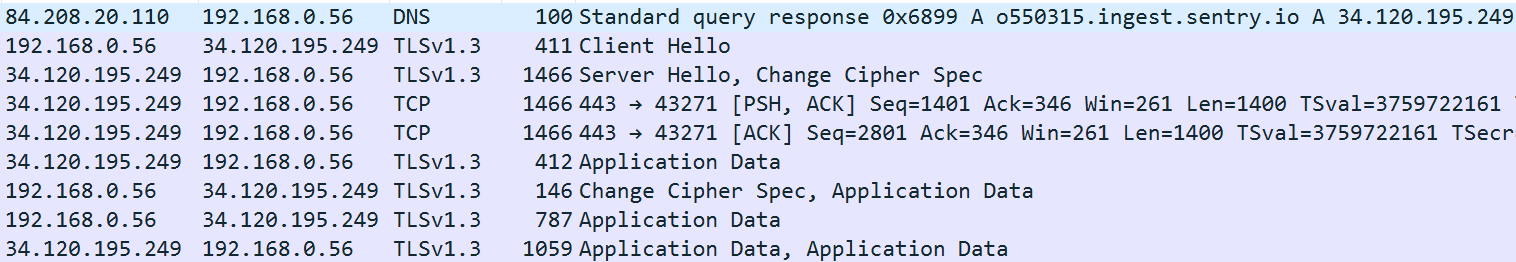
\includegraphics[width=\textwidth]{figures/irobot_AC_DNSimgset.png}
    \caption{TCP session between Irobot Roomba and \textit{0550315.ingest.sentry.io}, initiated after a cleaning is finished}
    \label{fig:AC_DNS_ingest}
\end{figure}


Calculations of number of bytes and  number of packets with associated average and \gls{SD} are presented in Table \ref{tab:ACoverallOSL} and Table \ref{tab:ACoverallDRA}. As presented, the average and standard deviation in Oslo environment is significantly higher than in Drammen, regardless of that the Drammen cleaning had a longer duration overall. This might be due to the number of obstacles or carpet in the environments. An interesting calculation is that more than 90\% of all packets captured are sent between the Irobot Roomba and \textit{s3.amazoneaws.com}, due to large packet sizes in the session this includes more than 95\% of the transferred bytes. \gls{TLS} encryption hides the information, but this is most likely an upload of all the cleaning data collected during the event, and if encryption is broken a lot of private information can be exposed. Event 6 in Oslo environment has a low number of bytes and packets compared to the other events, but included both \gls{DNS} responses and upload traffic associated with them. This could be due to lack of updates or disruption on transmission. 

\begin{table}[H]
\centering
\caption{Overall statistics for Automated Cleaning in Oslo}
\label{tab:ACoverallOSL}
\begin{tabular}{|c|c|c|}
\hline
\textbf{Event} & \textbf{Packet number} & \textbf{Total bytes sent} \\ \hline
Event 1        & 2,703                   & 3,882,164                   \\ \hline
Event 2        & 2,736                   & 3,811,206                   \\ \hline
Event 3        & 2,659                   & 3,818,287                   \\ \hline
Event 4        & 2,681                   & 3,747,788                   \\ \hline
Event 5        & 2,589                   & 3,704,329                   \\ \hline
Event 6        & 236                    & 237,163                    \\ \hline
Event 7        & 2,701                   & 3,860,634                   \\ \hline
Event 8        & 2,631                   & 3,770,236                   \\ \hline
Event 9        & 2,609                   & 3,738,406                   \\ \hline
Event 10       & 2,609                   & 3,799,896                   \\ \hline
Average        & 2,415.4                 & 3,437,010.9                 \\ \hline
SD       & 767.27
       & 1,125,643               \\ \hline
\end{tabular}
\end{table}

\begin{table}[H]
\centering
\caption{Overall statistics for Automated Cleaning in Drammen}
\label{tab:ACoverallDRA}
\begin{tabular}{|c|c|c|}
\hline
\textbf{Event} & \textbf{Packet number} & \textbf{Total bytes sent} \\ \hline
Event 1        & 1,074                   & 1,443,851                   \\ \hline
Event 2        & 1,131                   & 1,524,076                   \\ \hline
Event 3        & 1,209                   & 1,644,223                   \\ \hline
Event 4        & 1,207                   & 1,641,145                   \\ \hline
Event 5        & 1,013                   & 1,422,457                   \\ \hline
Event 6        & 1,013                   & 1,422,457                   \\ \hline
Event 7        & 1,220                   & 1,726,862                   \\ \hline
Event 8        & 1,248                   & 1,715,015                   \\ \hline
Event 9        & 1,227                   & 1,669,154                   \\ \hline
Event 10       & 1,456                   & 1,838,832                   \\ \hline
Average        & 1,179.8                 & 1,604,807.2                 \\ \hline
SD        & 131.48
       & 144,434.9               \\ \hline
\end{tabular}
\end{table}

The first 20 packet lengths in all event captures was extracted with a python script presented in Appendix \ref{app:Packetlengthex} and are analyzed to find common sequences that can be used to identify the event. These packet lengths are shown in Figure \ref{fig:ACseq}. D and S in front of the packet lengths indicates if the Irobot Roomba is destination or source of the packet. The yellow marked fields are the common identified sequence pattern in all event captures. The sequence starts with two packets sent from the Irobot cloud server to the Irobot Roomba with the lengths of \textit{315 or 316} and \textit{288 or 289} bytes, these two packets can be received in mixed order, but always appear as a packet pair. The Irobot Roomba then responded with a packet pair with lengths of \textit{176} and \textit{186 or 187} bytes. This is followed by a packet from the Irobot cloud server with the length of \textit{408 or 409} bytes. The entire identified packet sequence is therefore \textit{[315, 288, 176, 186, 408]} or \textit{[288, 315, 176, 186, 408]}, with a offset of 1 byte due to the variation of packet size within the sequence. Oslo event 2 and Drammen event 8 does not include this sequence, and it looks like one of the packet pairs are merged. 

\begin{figure}[H]
    \centering
    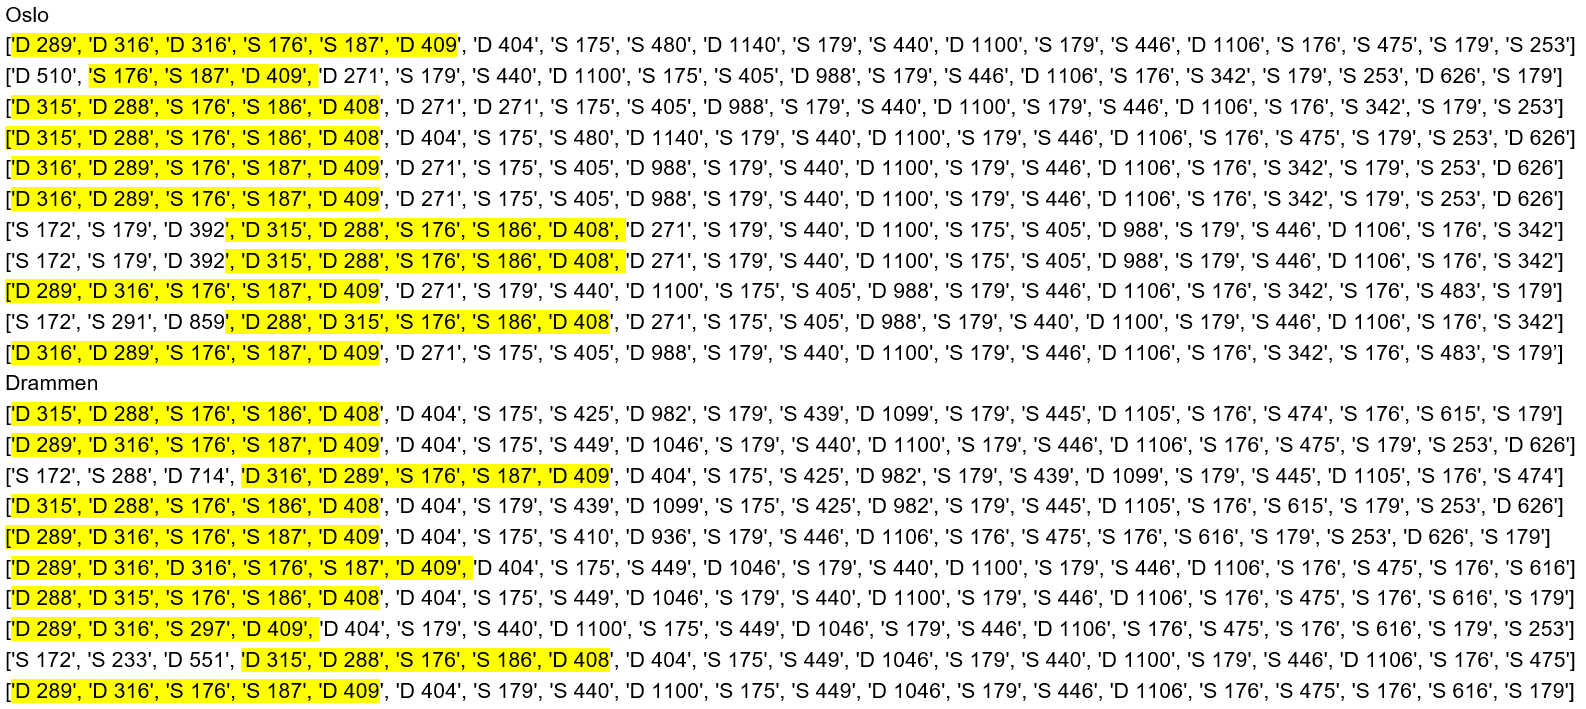
\includegraphics[width=\textwidth]{figures/Sequence_AC.png}
    \caption{Automated Cleaning extracted packet length sequences}
    \label{fig:ACseq}
\end{figure}

Both packet length sequences and the presence of two \gls{FQDN} are identified in all \textit{Automated cleaning} event captures. These observations forms the signature for this event. Two python functions were created: one for the detection of the \gls{DNS} responses for \textit{0550315.ingest.sentry.io} and \textit{s3.amazoneaws.com} and one to identify the packet sequences \textit{[315, 288, 176, 186, 408]} or \textit{[288, 315, 176, 186, 408]}. The pseudo code for \gls{DNS} detection is presented in Figure \ref{fig:pesudo_code_cleaning_event} and sequence detection in Figure \ref{fig:Pesudo_code_AC}.

\begin{figure}[H]
    \centering
    \begin{lstlisting}[numbers=left]
     function cleaning_event_detection(event_capture)
          if 'o550315.ingest.sentry.io' in event_capture
               dns1 == True
          elsif
               dns1 == False
          if 's3.amazonaws.com' in event_capture
               dns2 == True
          elsif
               dns2 == False
          if dns1 and dns2 == True      
               cleaning_confidence = + 10
          return cleaning_confidence
    \end{lstlisting}
    \caption{The algorithm for identifying \gls{DNS} responses for FQDNs \textit{0550315.ingest.sentry.io} and \textit{s3.amazoneaws.com}}
    \label{fig:pesudo_code_cleaning_event}
\end{figure}

\begin{figure}[H]
    \centering
    \begin{lstlisting}[numbers=left]
     function detect_application_start(packet_lengths_src)
          signature1 = [316, 289, 176, 187, 409]
          signature2 = [289, 316, 176, 187, 409]
          if signature1 in packet_lengths
               automated_cleaning_confidence = + 10
          elsif signature1 in packet_lengths
               automated_cleaning_confidence = + 10
    \end{lstlisting}
    \caption{The algorithm for identifying the \textit{Automated cleaning} packet length sequence}
    \label{fig:Pesudo_code_AC}
\end{figure}

To evaluate the detection algorithm it was used on all the different \textit{Automated cleaning} event files. The \gls{DNS} signature detection algorithm was able to identify the \gls{DNS} responses for \textit{0550315.ingest.sentry.io} and \textit{s3.amazoneaws.com} in all 20 event files. The sequence signature detection algorithm was able to identify the signature in 18 of 20 event files, resulting in a successful detection rate of 90\%. The two events that did not include this signature were Oslo event 2 and Drammen event 8, they had the sequences \textit{510, 176, 187, 409} and \textit{289, 316, 297, 409}. As mentioned in the sequence analysis the sequence detection will not be able to identify these.     

\section{Application Triggered Cleaning}

This section introduce specific configuration and decisions during the \textit{Application triggered cleaning} event triggering and analysis. The results from the analysis will be presented at the end of the section. 

\textit{Application triggered cleaning} is an event triggered manually by the Irobot Roomba's users through the Irobot home application's predefined or customized cleaning jobs. The event used a customized cleaning job defining the entire area of Oslo or Drammen smart map. This ensured that the cleaning area is constant for all the triggered events, creating the best foundation for comparison. These events can be triggered as many times as the user would like and is therefore the same during the entire capturing phase. 

Triggering date and time for all \textit{Application triggered cleaning} events are presented in Table \ref{tab:ATC_dateandtimeOslo} for Oslo and Table \ref{tab:ATC_dateandtimeDrammen} for Drammen. These events are triggered in a non-realistic manner due to time constrains, this is especially for the Drammen triggering where a new event was triggered every 30 minutes. In a realistic smart environment these triggerings would occur less and not in a structured manner. \textit{Application triggered cleaning} is triggered when the user needs additional cleaning outside of the scheduled one, preferably triggering this when leaving home. Identification of this event can therefore expose private information about user location. 

\begin{table}[H]
\centering
\caption{Application triggered cleaning triggering date and time overview for Oslo environment.}
\label{tab:ATC_dateandtimeOslo}
\begin{tabular}{|c|c|c|c|}
\hline
\textbf{Event} & \textbf{Date} & \textbf{Start time} & \textbf{End time} \\ \hline
1              & 28.02.2023         & 18:20               & 18:27             \\ \hline
2              & 28.02.2023         & 18:35               & 18:42             \\ \hline
3              & 01.03.2023         & 18:53               & 19:00             \\ \hline
4              & 09.03.2023         & 07:44               & 07:49             \\ \hline
5              & 09.03.2023         & 08:03               & 08:10             \\ \hline
6              & 09.03.2023         & 08:25               & 08:31             \\ \hline
7              & 09.03.2023         & 08:57               & 09:04             \\ \hline
8              & 09.03.2023         & 09:18               & 09:26             \\ \hline
9              & 12.03.2023         & 12:20               & 12:35             \\ \hline
10             & 12.03.2023         & 12:54               & 13:09             \\ \hline
\end{tabular}
\end{table}

\begin{table}[H]
\centering
\caption{Application triggered cleaning triggering date and time overview for Drammen environment.}
\label{tab:ATC_dateandtimeDrammen}
\begin{tabular}{|c|c|c|c|}
\hline
\textbf{Event} & \textbf{Date} & \textbf{Start time} & \textbf{End time} \\ \hline
1              & 25.02.2023         & 14:30               & 14:45             \\ \hline
2              & 25.02.2023         & 15:00               & 15:15             \\ \hline
3              & 25.02.2023         & 15:30               & 15:45             \\ \hline
4              & 25.02.2023         & 16:00               & 16:15             \\ \hline
5              & 25.02.2023         & 16:30               & 16:45             \\ \hline
6              & 25.02.2023         & 17:00               & 17:15             \\ \hline
7              & 25.02.2023         & 17:30               & 17:45             \\ \hline
8              & 25.02.2023         & 19:00               & 19:15             \\ \hline
9              & 25.02.2023         & 19:30               & 19:45             \\ \hline
10             & 25.02.2023         & 20:00               & 20:15             \\ \hline
\end{tabular}
\end{table}

Protocol distribution shows that there are two \gls{DNS} response packets in each of the event files, the rest of the traffic is \gls{TCP} where the majority are \gls{TLS} encrypted. \gls{TCP} packets without \gls{TLS} are either \gls{TCP} acknowledgement packets without payload or a part of a \gls{TCP} three-way-handshake or tare-down. When the event is triggered it is observed an increase in packets between the Irobot Roomba and the corresponding Irobot cloud server, this communication is at a consistent level until the cleaning is done. Then a \gls{DNS} response \gls{FQDN} \textit{0550315.ingest.sentry.io} is received and a new \gls{TCP} session to one of the responded \gls{IP} addresses is established. The entire corresponding \gls{TCP} session from Oslo environment event 5 is shown in Figure \ref{fig:ATC_DNS_ingest}, this is consistent for all \textit{Application triggered cleaning} events. After this session is finished a new \gls{DNS} response for \gls{FQDN} \textit{s3.amazoneaws.com} is received and a new \gls{TCP} session is established to one of the responded \gls{IP} addresses. 

\begin{figure}[H]
    \centering
    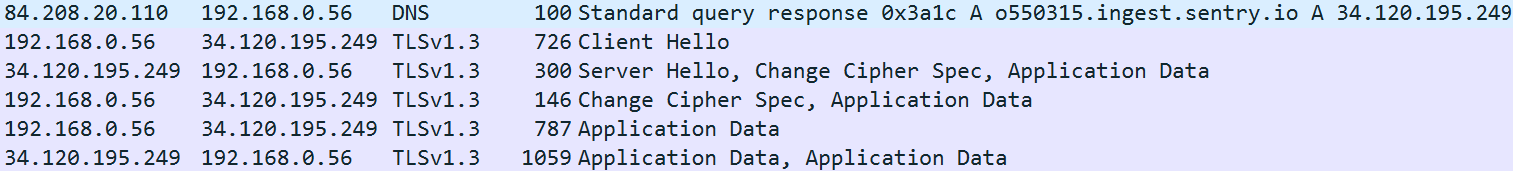
\includegraphics[width=\textwidth]{figures/irobot_ATC_DNSimgset.png}
    \caption{TCP session between Irobot Roomba and \textit{0550315.ingest.sentry.io}, initiated after application triggered cleaning is finished}
    \label{fig:ATC_DNS_ingest}
\end{figure}

Calculation of number of bytes and packets sent with associated average and standard deviation for all \textit{Application triggered cleaning} events are presented in Table \ref{tab:TCoverallOSL} and Table \ref{tab:TCoverallDRA}. Both number of packets and bytes sent are higher in Oslo despite shorter duration of cleaning, this could be environment specific due to floor, windows and furniture within each environment. More then 90\% of the packets are sent from the Irobot Roomba to \gls{FQDN} \textit{s3.amazoneaws.com}, as the majority of these packets are close to maximum packet size of 1,500 bytes they account for more then 95\% of the bytes transferred. This is most likely an upload of all the collected information form the cleaning. In Drammen environment both number of packets and bytes sent are increased for each consecutive event, based on similar duration and encrypted traffic it is not possible to determine why this occurred in Drammen. 

\begin{table}[H]
\centering
\caption{Application triggered cleaning, overall statistics Oslo}
\label{tab:TCoverallOSL}
\begin{tabular}{|c|c|c|}
\hline
\textbf{Event} & \textbf{Number of packets} & \textbf{Total number of bytes} \\ \hline
Event 1        & 2,667                   & 3,732,218                   \\ \hline
Event 2        & 2,686                   & 3,730,748                   \\ \hline
Event 3        & 2,656                   & 3,710,958                   \\ \hline
Event 4        & 3,065                   & 4,365,510                   \\ \hline
Event 5        & 2,880                   & 4,076,534                   \\ \hline
Event 6        & 2,633                   & 3,771,269                   \\ \hline
Event 7        & 2,661                   & 3,786,648                   \\ \hline
Event 8        & 2,647                   & 3,798,184                   \\ \hline
Event 9        & 2,729                   & 3,798,630                   \\ \hline
Event 10       & 2,639                   & 3,786,194                   \\ \hline
Average        & 2,726.3                 & 3,855,689.3                 \\ \hline
SD        & 139.57
       & 206,499.4               \\ \hline
\end{tabular}
\end{table}

\begin{table}[H]
\centering
\caption{Application triggered cleaning, overall statistics Drammen}
\label{tab:TCoverallDRA}
\begin{tabular}{|c|c|c|}
\hline
\textbf{Event} & \textbf{Number of packets} & \textbf{Number of bytes} \\ \hline
Event 1        & 708                    & 802,488                    \\ \hline
Event 2        & 724                    & 945,100                    \\ \hline
Event 3        & 740                    & 956,470                    \\ \hline
Event 4        & 809                    & 1,071,613                   \\ \hline
Event 5        & 824                    & 1,088,836                   \\ \hline
Event 6        & 869                    & 1,157,323                   \\ \hline
Event 7        & 855                    & 1,144,086                   \\ \hline
Event 8        & 929                    & 1,248,783                   \\ \hline
Event 9        & 988                    & 1,321,061                   \\ \hline
Event 10       & 983                    & 1,339,631                   \\ \hline
Average        & 842.9                  & 1,107,539.1                 \\ \hline
SD        & 101.85
       & 172,281.2               \\ \hline
\end{tabular}
\end{table}

The first 20 packet lengths of each of the \textit{Application triggered cleaning} events are extracted with the python script presented in Appendix \ref{app:Packetlengthex}. These sequences are manually analyzed to identify common packet length sequence to be used in event attribution. Packet lengths for all events are presented in Figure \ref{fig:ATCseq}, D and S indicate if the Irobot Roomba is destination or source of the packet. The yellow marked fields are the common sequences identified in the majority of event captures. Irobot cloud server is initiating the event with three packets with the length of \textit{[208, 288, 315]}, the last two packets can occur in mixed order, and all length can vary with one byte. Three packets are used to keep the complexity of the signature low. Identified sequence signature for \textit{Application triggered cleaning} is \textit{[208, 288, 315]} with the offset of 1 bytes for all packet sizes. Oslo event 9 is the only event capture wich does not include the identified signature, expected success rate of evaluation is therefore 95\%. 

\begin{figure}[H]
    \centering
    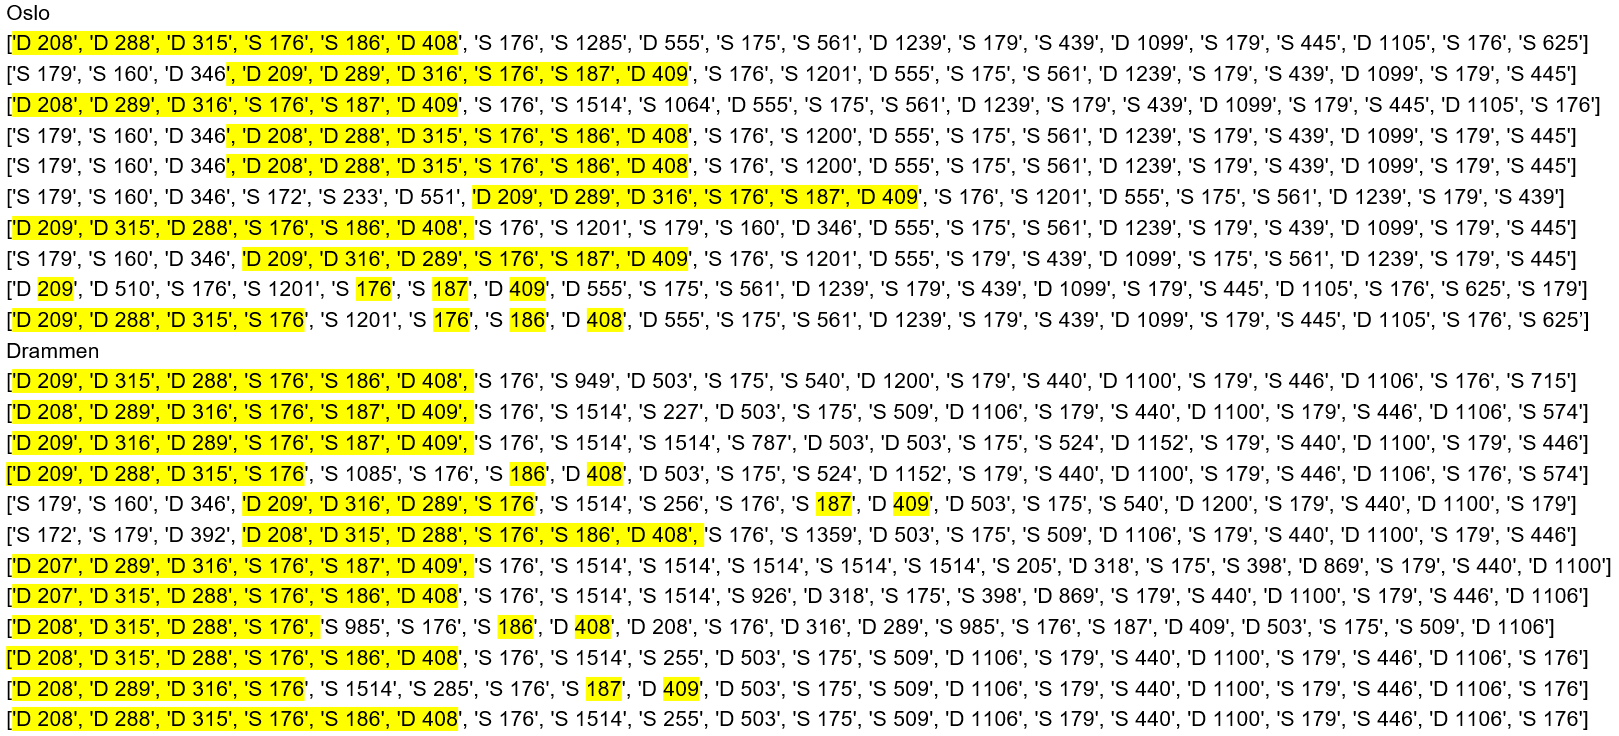
\includegraphics[width=\textwidth]{figures/Sequence_ATC.png}
    \caption{\textit{Application triggered} cleaning packet length sequence}
    \label{fig:ATCseq}
\end{figure}

To identify \textit{Application triggered cleaning} two detection algorithms are made, one identifying the \gls{DNS} responses \textit{0550315.ingest.sentry.io} and \textit{s3.amazoneaws.com} and one to identify the sequence signature specified above. Pseudo code for both algorithms are presented in Figure \ref{fig:pseudocodeATCDNS} and Figure \ref{fig:Sudo_code_ATC}.

\begin{figure}[H]
    \centering
    \begin{lstlisting}[numbers=left]
     function cleaning_event_detection(event_capture)
          if 'o550315.ingest.sentry.io' in event_capture
               dns1 == True
          elsif
               dns1 == False
          if 's3.amazonaws.com' in event_capture
               dns2 == True
          elsif
               dns2 == False
          if dns1 and dns2 == True      
               cleaning_confidence = + 10
          return cleaning_confidence
    \end{lstlisting}
    \caption{The algorithm for \gls{DNS} detection in Application triggered cleaning events}
    \label{fig:pseudocodeATCDNS}
\end{figure}

\begin{figure}[H]
    \centering
    \begin{lstlisting}[numbers=left]
     function detect_ATC(packet_lengths)
          signature1 = [209,289,316]
          signature2 = [209.316.289]
          if signature1 in packet_lengths
               ATC_confidence = + 10
          elsif signature1 in packet_lengths
              ATC_confidence = + 10
          return ATC_confidence
    \end{lstlisting}
    \caption{The algorithm for identifying the Application triggered cleaning packet sequence signature}
    \label{fig:Sudo_code_ATC}
\end{figure}

To evaluate the detection algorithms they are tested on all the capturing files for \textit{Application triggered cleaning}, trying to identify both signatures. The results of the identification are as expected,  \gls{DNS} detection had a success rate of 100\% and the sequence signature detection had a success rate of 95\%. The isolated event can therefore be identified with a high confidence, based on these results. 

\section{Scheduled Cleaning}
This section introduce specific configuration and decisions during \textit{Scheduled cleaning} event and analysis. The results from the analysis will be presented at the end of the section.

\textit{Scheduled cleaning} is triggered through configuration of customized cleaning jobs in the Irobot home application. A scheduled cleaning job was configured specifying the entire smart map as the cleaning area. Irobot restricts its users to not configure two scheduled cleanings with less then 3 hours space, cleaning jobs with less then 3 hours in between creates an error message. During this project only one scheduled clean was configured, but after the cleaning was finished the user entered the application changing the configured time. This enabled scheduled cleanings to be executed with less then 3 hours in between. It was observed that whenever a scheduled cleaning job was changed, the Irobot Roomba made a sound indicating that it got an update. The scheduled cleaning job is most likely sent to the vacuum cleaner at the time of configuration and then triggered locally. This way the Irobot Roomba is able to clean without Internet connection at the triggering time. 

Triggering dates and time for \textit{Scheduled cleaning} are presented in Table \ref{tab:SC_dateandtimeOslo} and \ref{tab:SC_dateandtimeDrammen}. These events are triggered in a non-realistic way due to time constrains, this is supported by Irobot's own restrictions mentioned above. Timings from \textit{Scheduled cleaning} can therefore not be used in the attribution of this specific event, however it would be a good indication if collected by an attack over a longer period of time. If a cleaning event is detected every Monday, Wednesday and Friday at 09:00 it is most likely due to scheduled cleaning, because a human triggered event would differ more in time. An observation during triggering was that the Irobot Roomba always started within 30 seconds before the scheduled time, this is also observed in the actual packet capture. In Figure \ref{fig:SC_start_time} event 2 in Oslo is shown, and there the traffic starts right before the scheduled timestamp. This is applicable for all events in the rage of 30-0 seconds before scheduled time. 

\begin{table}[H]
\centering
\caption{Scheduled cleaning triggering date and time overview for Oslo}
\label{tab:SC_dateandtimeOslo}
\begin{tabular}{|c|c|c|c|}
\hline
\textbf{Event} & \textbf{Date} & \textbf{Start time} & \textbf{End time} \\ \hline
1              & 10.03.2023         & 10:45               & 10:54             \\ \hline
2              & 10.03.2023         & 11:15               & 11:24             \\ \hline
3              & 10.03.2023         & 12:15               & 12:24             \\ \hline
4              & 10.03.2023         & 13:30               & 13:39             \\ \hline
5              & 10.03.2023         & 15:00               & 15:09             \\ \hline
6              & 10.03.2023         & 15:30               & 15:39             \\ \hline
7              & 10.03.2023         & 15:55               & 16:04             \\ \hline
8              & 10.03.2023         & 16:10               & 16:19             \\ \hline
9              & 11.03.2023         & 10:10               & 10:19             \\ \hline
10             & 11.03.2023         & 10:30               & 10:39             \\ \hline
\end{tabular}
\end{table}

\begin{table}[H]
\centering
\caption{Scheduled cleaning triggering date and time overview for Drammen}
\label{tab:SC_dateandtimeDrammen}
\begin{tabular}{|c|c|c|c|}
\hline
\textbf{Event} & \textbf{Date} & \textbf{Start time} & \textbf{End time} \\ \hline
1              & 25.02.2023         & 20:30               & 20:45             \\ \hline
2              & 25.02.2023         & 21:00               & 21:15             \\ \hline
3              & 26.02.2023         & 11:20               & 11:35             \\ \hline
4              & 26.02.2023         & 11:50               & 12:05             \\ \hline
5              & 26.02.2023         & 12:20               & 12:35             \\ \hline
6              & 26.02.2023         & 12:50               & 13:05             \\ \hline
7              & 26.02.2023         & 13:20               & 13:35             \\ \hline
8              & 26.02.2023         & 13:50               & 14:05             \\ \hline
9              & 26.02.2023         & 14:20               & 14:35             \\ \hline
10             & 26.02.2023         & 15:00               & 15:15             \\ \hline
\end{tabular}
\end{table}

\begin{figure}[H]
    \centering
    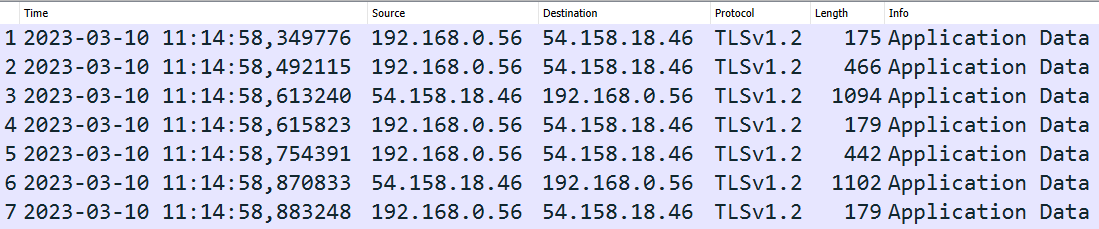
\includegraphics[width=\textwidth]{figures/SC_start_time.png}
    \caption{Start time for Scheduled cleaning in Oslo event 2, cleaning was scheduled 11:15}
    \label{fig:SC_start_time}
\end{figure}


Protocol distribution and overall traffic flow are similar as presented for \textit{Automated cleaning} and \textit{Application triggered cleaning}. The two same \gls{DNS} responses listed below are observed. 
\begin{itemize}
    \item 0550315.ingest.sentry.io
    \item s3.amazoneaws.com
\end{itemize}


Calculations of number of packets and bytes sent and \gls{SD} are presented in Table \ref{tab:scoverall} and Table \ref{tab:scoverallDRA}. Average and standard deviation in both Oslo and Drammen environment is small indicating small differences in the triggered events, this could be due to locally triggered events on the Irobot Roomba. 

\begin{table}[H]
\centering
\caption{Scheduled cleaning, overall statistics Oslo smart home}
\label{tab:scoverall}
\begin{tabular}{|c|c|c|}
\hline
\textbf{Event} & \textbf{Number of packets} & \textbf{Number of bytes} \\ \hline
Event 1        & 2,541                   & 3,669,941                   \\ \hline
Event 2        & 2,633                   & 3,678,959                   \\ \hline
Event 3        & 2,622                   & 3,660,004                   \\ \hline
Event 4        & 2,524                   & 3,629,262                   \\ \hline
Event 5        & 2,627                   & 3,658,515                   \\ \hline
Event 6        & 2,608                   & 3,729,110                   \\ \hline
Event 7        & 2,596                   & 3,645,238                   \\ \hline
Event 8        & 2,655                   & 3,685,536                   \\ \hline
Event 9        & 2,573                   & 3,713,211                   \\ \hline
Event 10       & 2,636                   & 3,768,883                   \\ \hline
Average        & 2,601.5                 & 3,683,865.9                 \\ \hline
SD       & 43.03       & 42,219.79               \\ \hline
\end{tabular}
\end{table}

\begin{table}[H]
\centering
\caption{Scheduled cleaning, overall statistics Drammen}
\label{tab:scoverallDRA}
\begin{tabular}{|c|c|c|}
\hline
\textbf{Event} & \textbf{Number of pkt} & \textbf{Number of bytes} \\ \hline
Event 1        & 996                    & 1,354,755                   \\ \hline
Event 2        & 1,052                   & 1,422,052                   \\ \hline
Event 3        & 1,150                   & 1,592,566                   \\ \hline
Event 4        & 1,317                   & 1,650,499                   \\ \hline
Event 5        & 1,166                   & 1,570,805                   \\ \hline
Event 6        & 1,179                   & 1,612,050                   \\ \hline
Event 7        & 1,160                   & 1,582,275                   \\ \hline
Event 8        & 1,177                   & 1,610,090                   \\ \hline
Event 9        & 1,205                   & 1,634,883                   \\ \hline
Event 10       & 1,170                   & 1,590,726                   \\ \hline
Average        & 1,157.2                 & 1,562,070.1                 \\ \hline
SD        & 85,66
       & 95,885,11               \\ \hline
\end{tabular}
\end{table}

The 20 first packet lengths were extracted with a python script presented in Appendix \ref{app:Packetlengthex}. The manual analysis of the packet lengths presented in Figure \ref{fig:Scseq}, resulted in two packet sequences of outbound traffic from the Irobot Roomba. The packet lengths varied more than previously and had a byte offset of 15 and 5 bytes depending on which signature sequence that was used. Both signature sequences are listed below with the associated byte offset. 

\begin{itemize}
    \item 176, 173, 179, 443, 177, byte offset 15 bytes 
    \item 176, 443, 179, 443, 177, byte offset 5 bytes
\end{itemize}

\begin{figure}[H]
    \centering
    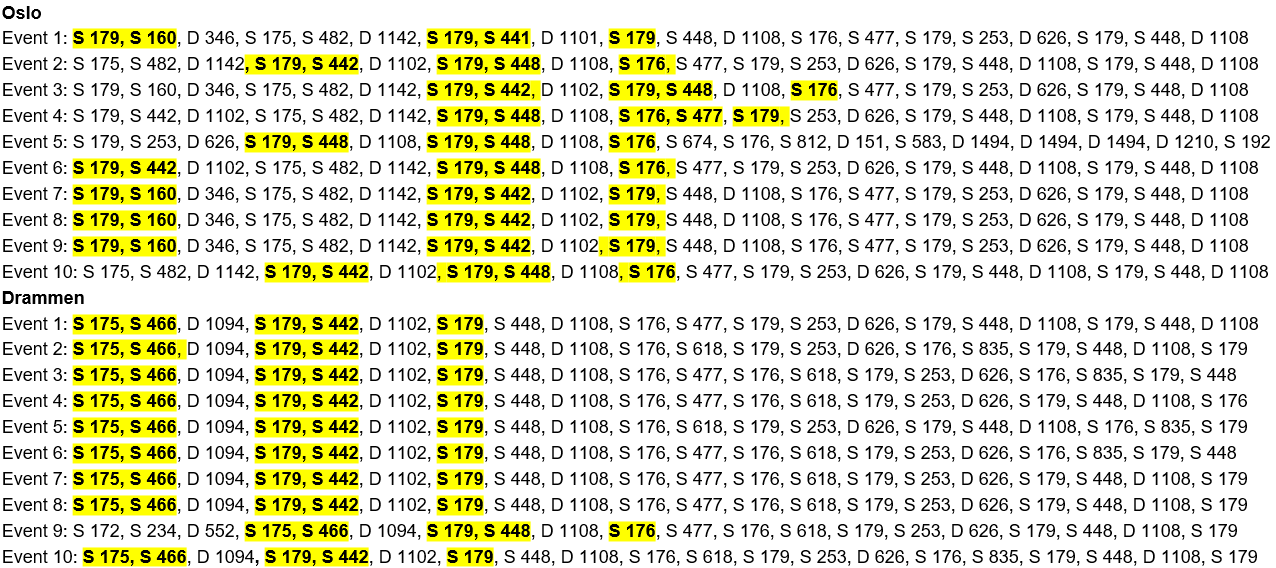
\includegraphics[width=\textwidth]{figures/Sequence_SC.png}
    \caption{\textit{Scheduled cleaning} packet length sequences}
    \label{fig:Scseq}
\end{figure}

As the \gls{DNS} signature is the same as for the two previous cleaning events analyzed, the same detection algorithm is used to evaluate this. Further, a new detection algorithm for the packet length sequence is presented in Figure \ref{fig:Sudo_code_SC_or_PC}. Both \gls{DNS} and sequence detection had a success rate of 100\% in all capturing files. Making this a good indication of the event if it is not detected in other events as well. 

\begin{figure}[H]
    \centering
    \begin{lstlisting}[numbers=left]
     function detect_application_start(packet_lengths_src)
          signature1 = [176,173,179,443,177]
          signature2 = = [176,443,179,443,177]
          if signature1 in packet_lengths
               SC_PTC_confidence = + 10
          elsif signature1 in packet_lengths
               SC_PTC_confidence = + 10
          return SC_PTC_confidence
    \end{lstlisting}
    \caption{Algorithm for scheduled cleaning packet sequence signature detection}
    \label{fig:Sudo_code_SC_or_PC}
\end{figure}


\section{Physical Triggered Cleaning}
This section introduce specific configuration and decisions during \textit{Physical triggered cleaning} event and analysis. The results from the analysis will be presented at the end of the section.

\textit{Physical triggered cleaning} events are only triggered by pressing the physical button on the Irobot Roomba. During triggering the user had to press the button twice to start the cleaning. Event triggering dates and time are presented in Table \ref{tab:PTC_dateandtimeOslo} and Table \ref{tab:PTC_dateandtimeDrammen}. The triggering in Oslo appears more realistic due to Drammen's strict triggering plan, these timestamps can therefore not be used to differentiate different cleaning events, but could have been a good indication if captured in a real-life smart environment. 

\begin{table}[H]
\centering
\caption{Physical triggered cleaning date and time overview for Oslo}
\label{tab:PTC_dateandtimeOslo}
\begin{tabular}{|c|c|c|c|}
\hline
\textbf{Event} & \textbf{Date} & \textbf{Start time} & \textbf{End time} \\ \hline
1              & 23.02.2023         & 18:08               & 18:24             \\ \hline
2              & 23.02.2023         & 18:36               & 19:05             \\ \hline
3              & 23.02.2023         & 19:14               & 19:34             \\ \hline
4              & 23.02.2023         & 20:13               & 20:35             \\ \hline
5              & 23.02.2023         & 20:44               & 21:06             \\ \hline
6              & 09.03.2023         & 09:43               & 10:02             \\ \hline
7              & 09.03.2023         & 10:30               & 10:50             \\ \hline
8              & 09.03.2023         & 12:32               & 12:50             \\ \hline
9              & 09.03.2023         & 13:16               & 14:05             \\ \hline
10             & 09.03.2023         & 17:44               & 18:05             \\ \hline
\end{tabular}
\end{table}

\begin{table}[H]
\centering
\caption{Physical triggered cleaning date and time overview for Drammen}
\label{tab:PTC_dateandtimeDrammen}
\begin{tabular}{|c|c|c|c|}
\hline
\textbf{Event} & \textbf{Date} & \textbf{Start time} & \textbf{End time} \\ \hline
1              & 25.02.2023         & 22:00               & 22:12             \\ \hline
2              & 25.02.2023         & 22:30               & 22:45             \\ \hline
3              & 25.02.2023         & 23:00               & 23:15             \\ \hline
4              & 25.02.2023         & 23:20               & 23:35             \\ \hline
5              & 25.02.2023         & 23:40               & 23:55             \\ \hline
6              & 26.02.2023         & 00:00               & 00:15             \\ \hline
7              & 26.02.2023         & 00:20               & 00:35             \\ \hline
8              & 26.02.2023         & 00:40               & 00:55             \\ \hline
9              & 26.02.2023         & 01:06               & 01:20             \\ \hline
10             & 26.02.2023         & 01:31               & 01:45             \\ \hline
\end{tabular}
\end{table}

Protocol distribution and traffic flow are similar as in the other three cleanings events presented above. The two same \gls{DNS} responses are identified as well as their corresponding \gls{TCP} sessions. Standard deviation for both environments are small, indicating that the events are similar and supporting that the hypothesis on 20 events are sufficient. 

\begin{table}[H]
\centering
\caption{Physical triggered cleaning, overall statistics Oslo}
\label{tab:PCoverallOSL}
\begin{tabular}{|c|c|c|}
\hline
\textbf{Event} & \textbf{Number of packets} & \textbf{Number of bytes} \\ \hline
Event 1        & 2,791                   & 3,965,147                   \\ \hline
Event 2        & 3,180                   & 4,357,126                   \\ \hline
Event 3        & 2,926                   & 4,033,946                   \\ \hline
Event 4        & 2,872                   & 4,112,516                   \\ \hline
Event 5        & 2,944                   & 4,209,443                   \\ \hline
Event 6        & 2,984                   & 4,122,412                   \\ \hline
Event 7        & 2,925                   & 4,160,462                   \\ \hline
Event 8        & 2,869                   & 4,100,166                   \\ \hline
Event 9        & 2,918                   & 4,227,626                   \\ \hline
Event 10       & 2,768                   & 3,957,559                   \\ \hline
Average        & 2,917.7                 & 4,124,640.3                 \\ \hline
SD        & 113.98
       & 122,683.4               \\ \hline
\end{tabular}
\end{table}

\begin{table}[H]
\centering
\caption{Physical triggered cleaning, overall statistics Drammen}
\label{tab:PCoverallDRA}
\begin{tabular}{|c|c|c|}
\hline
\textbf{Event} & \textbf{Number of packets} & \textbf{NUmber of bytes} \\ \hline
Event 1        & 1,078                   & 1,481,677                   \\ \hline
Event 2        & 1,087                   & 1,484,930                   \\ \hline
Event 3        & 1,125                   & 1,520,872                   \\ \hline
Event 4        & 1,088                   & 1,517,429                   \\ \hline
Event 5        & 1,150                   & 1,555,605                   \\ \hline
Event 6        & 1,086                   & 1,507,084                   \\ \hline
Event 7        & 1,092                   & 1,501,894                   \\ \hline
Event 8        & 1,115                   & 1,510,971                   \\ \hline
Event 9        & 1,098                   & 1,485,863                   \\ \hline
Event 10       & 1,100                   & 1,492,331                   \\ \hline
Average        & 1,101.9                 & 1,505,865.6                 \\ \hline
SD        &22.05
       & 22,318.19               \\ \hline
\end{tabular}
\end{table}

The first 20 packet lengths are extracted with the same python script as for the other events, presented in Appendix \ref{app:Packetlengthex}. Analysis resulted in the identification of the same packet sequence as for \textit{Scheduled cleaning} event, this could be because these two events are both triggered on the Irobot Roomba locally and not initiated from the Irobot cloud server. If this is the reason, the identified sequence could be present in all cleaning events. The extracted sequences are presented in Figure \ref{fig:PCseq}, yellow marked are the identified sequence and D and S represents if the Irobot Roomba is destination or source of the packet. 

\begin{figure}[H]
    \centering
    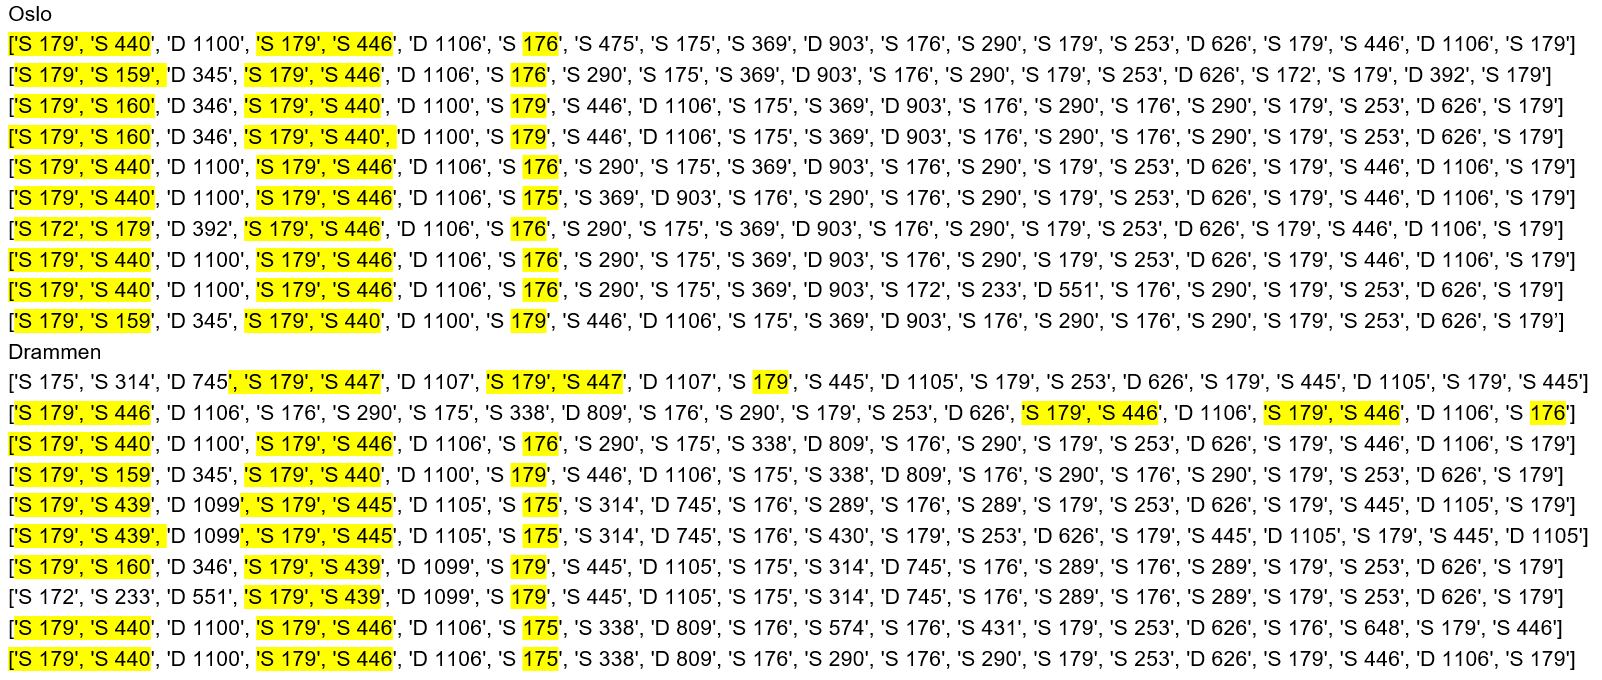
\includegraphics[width=\textwidth]{figures/Sequence_PC.png}
    \caption{Physical triggered cleaning packet length sequences}
    \label{fig:PCseq}
\end{figure}

The identified signatures are identical as for \textit{Scheduled cleaning}, the two same signature detection algorithms were used to evaluate the findings. Both algorithms had a 100\% success rate for identifying \textit{Physical triggered cleaning}, this means that neither of the events can be distinguished with these signatures. This attribution could been done by using timestamps, but the events in this research have too unrealistic triggering. 

\section{Application Start}
This section introduce specific configuration and decisions during \textit{Application start} event and analysis. The results from the analysis will be presented at the end of the section.

\textit{Application start} events are triggered by the user opening the Irobot application. Triggering dates and times are presented in Table \ref{tab:AS_dateandtimeOslo} and Table \ref{tab:AS_dateandtimeDrammen}. No specific action was defined during the event, so several different actions was executed such as, changing scheduled cleaning time, watch the dashboard and display configuration. Only the initial event traffic will therefore be included in the application open event. 

\begin{table}[H]
\centering
\caption{Application start event date and time overview for Oslo}
\label{tab:AS_dateandtimeOslo}
\begin{tabular}{|c|c|c|c|}
\hline
\textbf{Event} & \textbf{Date} & \textbf{Start time} & \textbf{End time} \\ \hline
1              & 10.03.2023         & 10:26               & 10:27             \\ \hline
2              & 10.03.2023         & 11:06               & 11:07             \\ \hline
3              & 10.03.2023         & 11:56               & 11:57             \\ \hline
4              & 10.03.2023         & 13:22               & 13:23             \\ \hline
5              & 10.03.2023         & 14:58               & 14:59             \\ \hline
6              & 10.03.2023         & 15:27               & 15:28             \\ \hline
7              & 10.03.2023         & 15:51               & 15:52             \\ \hline
8              & 10.03.2023         & 16:07               & 16:08             \\ \hline
9              & 11.03.2023         & 10:06               & 10:07             \\ \hline
10             & 11.03.2023         & 10:22               & 10:23             \\ \hline
\end{tabular}
\end{table}

\begin{table}[H]
\centering
\caption{Application start event date and time overview for Drammen}
\label{tab:AS_dateandtimeDrammen}
\begin{tabular}{|c|c|c|c|}
\hline
\textbf{Event} & \textbf{Date} & \textbf{Start time} & \textbf{End time} \\ \hline
1              & 25.02.2023         & 20:50               & 20:52             \\ \hline
2              & 25.02.2023         & 21:20               & 21:21             \\ \hline
3              & 25.02.2023         & 22:20               & 22:22             \\ \hline
4              & 25.02.2023         & 22:50               & 22:52             \\ \hline
5              & 26.02.2023         & 11:10               & 11:11             \\ \hline
6              & 26.02.2023         & 11:40               & 11:41             \\ \hline
7              & 26.02.2023         & 12:10               & 12:11             \\ \hline
8              & 26.02.2023         & 12:40               & 12:41             \\ \hline
9              & 26.02.2023         & 13:10               & 13:11             \\ \hline
10             & 26.02.2023         & 13:40               & 13:41             \\ \hline
\end{tabular}
\end{table}

The protocol distribution analysis identified only \gls{TCP} packets, no \gls{DNS} packets is sent during the event, indication that the requested information pulled from the Irobot Roomba when the application is started is initiated from \textit{a2uowfjvhio0fa.iot.us-east-1.amazonaws.com}. If the smart phone had been located in the same smart environment, it could be possible to identify a \gls{DNS} request to this service. No standard action was performed in the application during this event, the standard deviation from the calculations presented in Table \ref{tab:ASoverallOslo} and Table \ref{tab:ASoverallDRA} is therefore large, and only the initiating traffic is relevant to this analysis. During event 5-10 in Drammen, the user performed a scheduled clean configuration resulting in a high number of bytes sent compared to some of the other events.  

\begin{table}[H]
\centering
\caption{Application start event overall statistics Oslo}
\label{tab:ASoverallOslo}
\begin{tabular}{|l|l|l|}
\hline
\textbf{Event} & \textbf{Number of packets} & \textbf{Number of bytes} \\ \hline
Event 1        & 11                     & 5,202                      \\ \hline
Event 2        & 22                     & 8,698                      \\ \hline
Event 3        & 20                     & 8,644                      \\ \hline
Event 4        & 17                     & 7,135                      \\ \hline
Event 5        & 20                     & 8,580                      \\ \hline
Event 6        & 20                     & 8,608                      \\ \hline
Event 7        & 20                     & 9,213                      \\ \hline
Event 8        & 23                     & 9,527                      \\ \hline
Event 9        & 20                     & 8,730                      \\ \hline
Event 10       & 19                     & 8,877                      \\ \hline
Average        & 19.2                   & 8,321.4                    \\ \hline
SD        & 3.29
       & 1,258.62               \\ \hline
\end{tabular}
\end{table}

\begin{table}[H]
\centering
\caption{Application start, overall statistics Drammen}
\label{tab:ASoverallDRA}
\begin{tabular}{|l|l|l|}
\hline
\textbf{Event} & \textbf{Packet number} & \textbf{Total bytes sent} \\ \hline
Event 1        & 30                     & 20,875                     \\ \hline
Event 2        & 26                     & 19,568                     \\ \hline
Event 3        & 8                      & 2,655                      \\ \hline
Event 4        & 8                      & 2,659                      \\ \hline
Event 5        & 26                     & 19,561                     \\ \hline
Event 6        & 34                     & 21,897                     \\ \hline
Event 7        & 29                     & 20,222                     \\ \hline
Event 8        & 25                     & 19,468                     \\ \hline
Event 9        & 33                     & 21,744                     \\ \hline
Event 10       & 26                     & 19,570                     \\ \hline
Average        & 24,5                   & 16,821.9                   \\ \hline
SD       & 9.22
       & 7.519.30               \\ \hline
\end{tabular}
\end{table}

The first 20 packet lengths were extracted with the python script presented in Appendix \ref{app:Packetlengthex}, and the result is presented in Figure \ref{fig:ASseq}. The yellow marked fields are a part of the identified packet length sequence. The identified sequences are \textit{[209, 288, 315]} and \textit{[209, 315, 288]}, where both sequences have an offset of 1 byte. This is the same packet sequence signature as identified in \textit{Application triggered cleaning}, and is therefore used to identify \textit{Application start}. These sequences are therefore generated whenever the Irobot home application is started. To differentiate these two events the \gls{DNS} signature found in all cleaning events have to be identified.  

\begin{figure}[H]
    \centering
    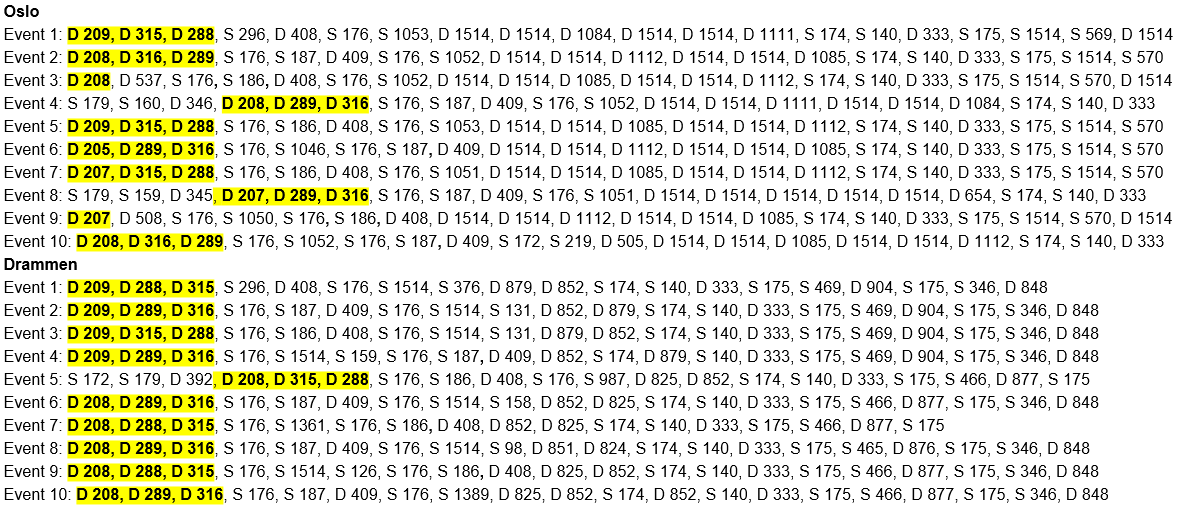
\includegraphics[width=\textwidth]{figures/Sequence_AS.png}
    \caption{Application start packet length sequences}
    \label{fig:ASseq}
\end{figure}

Evaluation of \textit{Application start} detection is determined with the same packet length sequence detection algorithm presented in Figure \ref{fig:Sudo_code_ATC}. This detection had a success rate of 90\% detection of the event, and it is therefore possible to determine that the application is started with high confidence.

\section{Bin Remove}
This section introduce specific configuration and decisions during \textit{Bin remove} event and analysis. The results from the analysis will be presented at the end of the section.

\textit{Bin remove} is triggered when the physical bin eject button is pressed on the Irobot Roomba i7 and the bin is then released. It is injected by pushing the bin back into place. Triggering dates and times are presented in Table \ref{tab:BR_dateandtimeOslo} and \ref{tab:BR_dateandtimeDrammen}, intervals between the triggering is small, but in analysis it was possible to differentiate when the different traffic occurred. During event triggering the response from the Irobot Roomba was variable, sometimes it flashed and sometimes it did not respond at all. The flashing is due to the Irobot Roomba loosing connection to the charger and not ejection of the bin. The amount of packets and bytes are also variable most likely due to the inconsistent in the event triggering process, resulting in a high standard deviation. These calculations are presented in Table \ref{tab:BRoverallOslo} and Table \ref{tab:BRoverallDRA}. 

\begin{table}[H]
\centering
\caption{Bin remove date and time overview for Oslo}
\label{tab:BR_dateandtimeOslo}
\begin{tabular}{|c|c|c|c|}
\hline
\textbf{Event} & \textbf{Date} & \textbf{Start time} & \textbf{End time} \\ \hline
1              & 11.03.2023    & 17:30               & 17:31             \\ \hline
2              & 11.03.2023    & 17:35               & 17:36             \\ \hline
3              & 11.03.2023    & 17:40               & 17:41             \\ \hline
4              & 11.03.2023    & 17:44               & 17:45             \\ \hline
5              & 11.03.2023    & 17:47               & 17:48             \\ \hline
6              & 11.03.2023    & 17:49               & 17:50             \\ \hline
7              & 11.03.2023    & 17:51               & 17:52             \\ \hline
8              & 11.03.2023    & 17:53               & 17:54             \\ \hline
9              & 11.03.2023    & 17:55               & 17:56             \\ \hline
10             & 11.03.2023    & 18:01               & 18:02             \\ \hline
\end{tabular}
\end{table}

\begin{table}[H]
\centering
\caption{Bin remove date and time overview for Drammen}
\label{tab:BR_dateandtimeDrammen}
\begin{tabular}{|c|c|c|c|}
\hline
\textbf{Event} & \textbf{Date} & \textbf{Start time} & \textbf{End time} \\ \hline
1              & 26.02         & 15:22               & 15:23             \\ \hline
2              & 26.02         & 15:30               & 15:31             \\ \hline
3              & 26.02         & 15:35               & 15:36             \\ \hline
4              & 27.02         & 15:05               & 15:06             \\ \hline
5              & 27.02         & 15:10               & 15:11             \\ \hline
6              & 27.02         & 15:15               & 15:16             \\ \hline
7              & 27.02         & 15:20               & 15:21             \\ \hline
8              & 27.02         & 15:25               & 15:26             \\ \hline
9              & 27.02         & 15:30               & 15:31             \\ \hline
10             & 27.02         & 15:35               & 15:36             \\ \hline
\end{tabular}
\end{table}

\begin{table}[H]
\centering
\caption{Bin remove, overall statistics Oslo}
\label{tab:BRoverallOslo}
\begin{tabular}{|l|l|l|}
\hline
\textbf{Event} & \textbf{Packet number} & \textbf{Total bytes sent} \\ \hline
Event 1        & 6                      & 2,512                      \\ \hline
Event 2        & 15                     & 5,765                      \\ \hline
Event 3        & 12                     & 4,366                      \\ \hline
Event 4        & 15                     & 7,869                      \\ \hline
Event 5        & 12                     & 5,022                      \\ \hline
Event 6        & 17                     & 8,426                      \\ \hline
Event 7        & 18                     & 8,492                      \\ \hline
Event 8        & 12                     & 5,022                      \\ \hline
Event 9        & 11                     & 4,956                      \\ \hline
Event 10       & 12                     & 5,022                      \\ \hline
Average        & 13                     & 5,745.2                    \\ \hline
SD        & 3.43
       & 1,937.64               \\ \hline
\end{tabular}
\end{table}


\begin{table}[H]
\centering
\caption{Bin remove, overall statistics Drammen }
\label{tab:BRoverallDRA}
\begin{tabular}{|l|l|l|}
\hline
\textbf{Event} & \textbf{Packet number} & \textbf{Total bytes sent} \\ \hline
Event 1        & 23                     & 8,610                      \\ \hline
Event 2        & 24                     & 10,149                     \\ \hline
Event 3        & 9                      & 4,407                      \\ \hline
Event 4        & 12                     & 5,022                      \\ \hline
Event 5        & 8                      & 4,333                      \\ \hline
Event 6        & 9                      & 4,399                      \\ \hline
Event 7        & 17                     & 6,595                      \\ \hline
Event 8        & 9                      & 4,399                      \\ \hline
Event 9        & 15                     & 7,869                      \\ \hline
Event 10       & 12                     & 5,022                      \\ \hline
Average        & 13,8                   & 6,080.5                    \\ \hline
SD        & 5.87
       & 2,112.52               \\ \hline
\end{tabular}
\end{table}

Packet length sequences were extracted with the python script in Appendix \ref{app:Packetlengthex}, and the results are presented in Figure \ref{fig:BRseq}. The identified sequences are marked in yellow, packets with the length of \textit{410 or 411} bytes were observed, these lengths are not observed in other events and is defined as the sequence signature for \textit{Bin remove}. The detection algorithm created is presented in pseudo code in Figure \ref{fig:Sudo_code_BinRemove} and is used to identify the signature in all event capture files. The evaluation result of testing is 100\% success rate of signature detection.   

\begin{figure}[H]
    \centering
    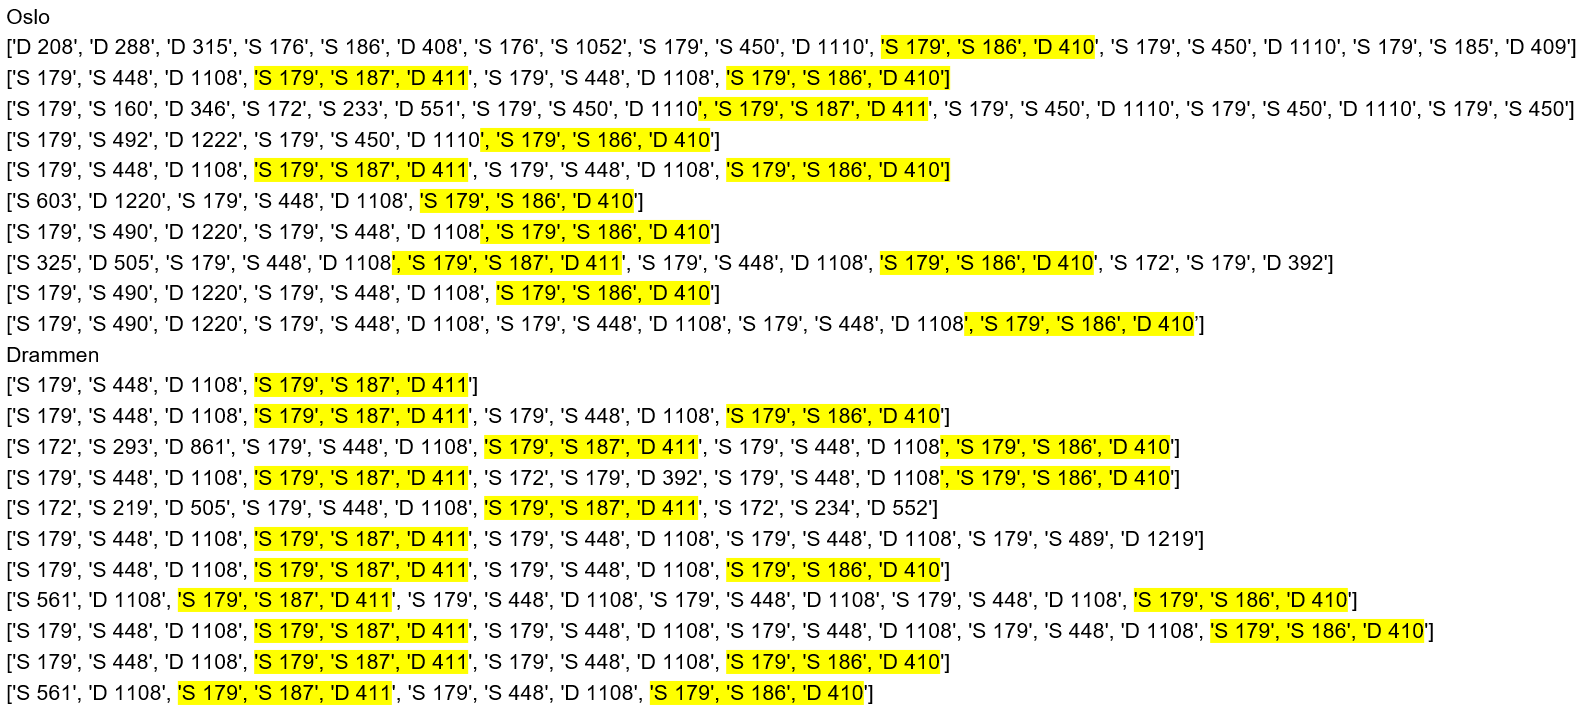
\includegraphics[width=\textwidth]{figures/Sequence_BR.png}
    \caption{Bin remove packet length sequences}
    \label{fig:BRseq}
\end{figure}

\begin{figure}[H]
    \centering
    \begin{lstlisting}[numbers=left]
     function bin_remove(br_confidence)
          if packet.length == 410 or 411 in capture.file
              br_confident = + 10
          return br_confident
    \end{lstlisting}
    \caption{Pseudo code for detection algorithm for \textit{Physical triggered cleaning} packet length sequence}
    \label{fig:Sudo_code_BinRemove}
\end{figure}

\section{Signature Comparison}
This section will present the comparison of the different signatures used for event attribution in the sections above. First an evaluation test where all signatures are tested on all events to identify if the signatures are unique. This is followed by an analysis of the evaluation results.

 \textit{Remove bin} signature seems to be detected in all events except \textit{Application start}, this signature is therefore removed from further analysis. 

All the different cleaning events, \textit{Automated cleaning, Scheduled cleaning, Application triggered cleaning} and \textit{Physical triggered cleaning} had the same \gls{DNS} responses present in the packet capturing. First a \gls{DNS} response for \gls{FQDN} \textit{0550315.ingest.sentry.io}, followed by a response for\textit{s3.amasoneaws.com}. These \gls{DNS} packets can therefore not be used as signature for any of the specific cleaning events, but can increase confidence in a cleaning detection. However there are several similarities between the identified sequences and this will be discussed further.

Signature sequence can not differentiate between \textit{Scheduled cleaning} or \textit{Physical triggered cleaning}. However the traffic sequence on all the scheduled cleaning events is started within a minute before the scheduled cleaning's configured triggering time. It is safe to assume that scheduled cleaning is configured every whole hour or half hour. A normal user would not configure a cleaning at 15:17, but more likely at 15:00. If an attacker is monitoring a smart environment during a longer time period, the two different cleanings can be separated based on reoccurring identification. A identified cleaning every Monday at 07:59 is most likely a scheduled cleaning, since humans are unable to provide the same level of consistency as \gls{IoT} devices.

We can assume that the sequence used to identify \textit{Application triggered cleaning} and \textit{Application start} is due to the fact that the application is started, and not the actual triggering of the cleaning event. It is still possible to differentiate between these two events with the use of cleaning \gls{DNS} signature. As all other cleaning events, it includes a \gls{DNS} response for \gls{FQDN} \textit{0550315.ingest.sentry.io} and then \textit{s3.amazoneaws.com}. If the \textit{Application start} sequences and the cleaning \gls{DNS} responses are detected, an application triggered cleaning is most likely executed. An element of uncertainty occurs if the user opens the application before or during another cleaning event, then this could create a false positive. 

The only difference between \textit{Automated cleaning} and \textit{Application triggered cleaning} is the first package in the sequence of \textit{Application start}. This packet has the length of 209 or 208 bytes and occurs every time the application is started. The identification of this is therefore a good attribute to differentiate for these events.

\section{Wireless and Wired Traffic Capture Comparison}
This section will compare the corresponding \gls{LAN} and \gls{WLAN} captures, and determine if the same method and identification can be applicable to identify events only based on wireless traffic as well. 

\gls{WLAN} and \gls{LAN} traffic were captured for all triggered events, but due to the thesis' time constrains only identification of signatures and detection algorithms on \gls{LAN} captures was conducted. The simulated \gls{WAN} traffic had more available attributes, due to the \gls{Wi-Fi}'s encryption. In  \cite{pingpong_trimananda2020packet} they have already proposed a method to identify actions based on packet lengths. This research therefore focused on the \gls{WAN} traffic, to be able to include \gls{DNS} as an identifier. To evaluate if the same method and algorithms are applicable to \gls{WLAN} traffic a comparison of two corresponding captures was done. Through analysis we identified that the added \gls{Wi-Fi} header was 79 bytes and the base filter of 97 bytes in \gls{LAN} captures was therefore converted to 176 bytes in \gls{WLAN}. When this filter was applied, the same packet sequences as in the simulated \gls{WAN} traffic were observed. These findings are presented in Figure \ref{fig:WLANLANHeader}. With the basefilter applied, it was observed that the \gls{WLAN} capture included less packets than the corresponding \gls{LAN} capture. This could be the result of retransmission, dual \gls{Wi-Fi} channels, signal disruption or packet collision on the \gls{NIC} in monitoring mode. When the \gls{NIC} was configured in monitoring mode, it collected all \gls{Wi-Fi} traffic in the area. This includes traffic from other \gls{SSID}s within wireless coverage. The original \gls{ISP} modem was also broadcasting it's \gls{SSID}s, causing high Signal to Noise Ratio (SnR) for more than one \gls{SSID}. Without control traffic between the \gls{AP} and the \gls{NIC} it could potentially lose traffic. Regardless of the packet loss it is still possible to identify similar patterns in \gls{WLAN} traffic as in \gls{LAN} traffic. 

\begin{figure}[H]
    \centering
    \begin{subfigure}[b]{0.9\textwidth}
        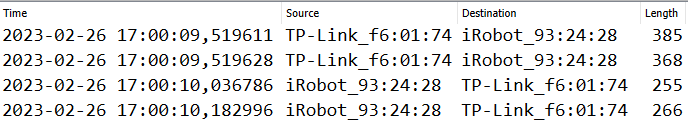
\includegraphics[width=\textwidth]{figures/WLANLANComparison.png}
        \caption{\gls{WLAN}}
    \end{subfigure}
    \quad
    \begin{subfigure}[b]{0.9\textwidth}
        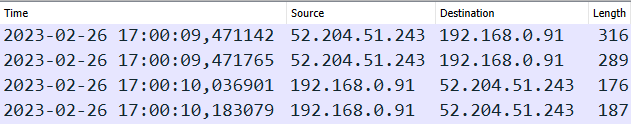
\includegraphics[width=\textwidth]{figures/LANWLANcomparison.png}
        \caption{\gls{LAN}}
    \end{subfigure}
    
    \caption{\gls{WLAN} and \gls{LAN} comparison}
    \label{fig:WLANLANHeader}
\end{figure}

\gls{WLAN} captures need more analysis before they can be implemented in the detection algorithm. An advantage of \gls{WLAN} traffic is the availability of \gls{MAC} addresses, an attacker can therefore easily identify the robot vacuum cleaner and filter traffic based on this information. Compared to \gls{LAN} where an attacker will have to eavesdrop for up to 24 hours before the Irobot traffic can be identified. 

Number of packets or bytes transmitted could also be used as an attribute to identify that there has been triggered a cleaning within the smart environment. This detection will be applicable for both \gls{LAN} and \gls{WLAN} eavesdropping.  
\chapter{Evaluation}
\label{cap:Evaluation}
This chapter will evaluate the performance of each event identification algorithm that we presented in the last chapter.


\section{Evaluation Method}
This section describes the method used to evaluate the thesis results. The evaluation process reuse network infrastructure, capturing process and data filtering as in the original research. Some new aspects are included in the evaluation to make the environments more representative for smart environments. These new aspects are describes in detail further in this section.

\subsubsection{Evaluation environments}
Event triggering during evaluation was conducted in three different environments, now called Guestroom, Bedroom and Living room. Environment layout is shown in Figure \ref{fig:Liveroom}. The Irobot Roomba i7 was reverted to factory default for each of the evaluation environments, this mitigates the change of any interference between the environments. User input such as robot, floor and room names was configured differently for all environments. A map discovery process was executed as part of the inital set-up phase.

\begin{figure}[H]
    \centering
    
    \begin{subfigure}{0.35\textwidth}
        \centering
        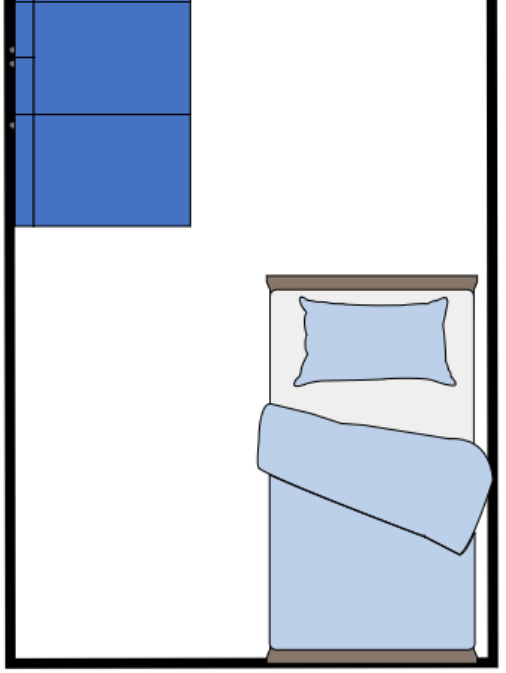
\includegraphics[width=\linewidth]{figures/Liveroom1.png}
        \caption{Guestroom evaluation environment}
        \label{fig:Liveroom1}
    \end{subfigure}
    \hfill
    \begin{subfigure}{0.35\textwidth}
        \centering
        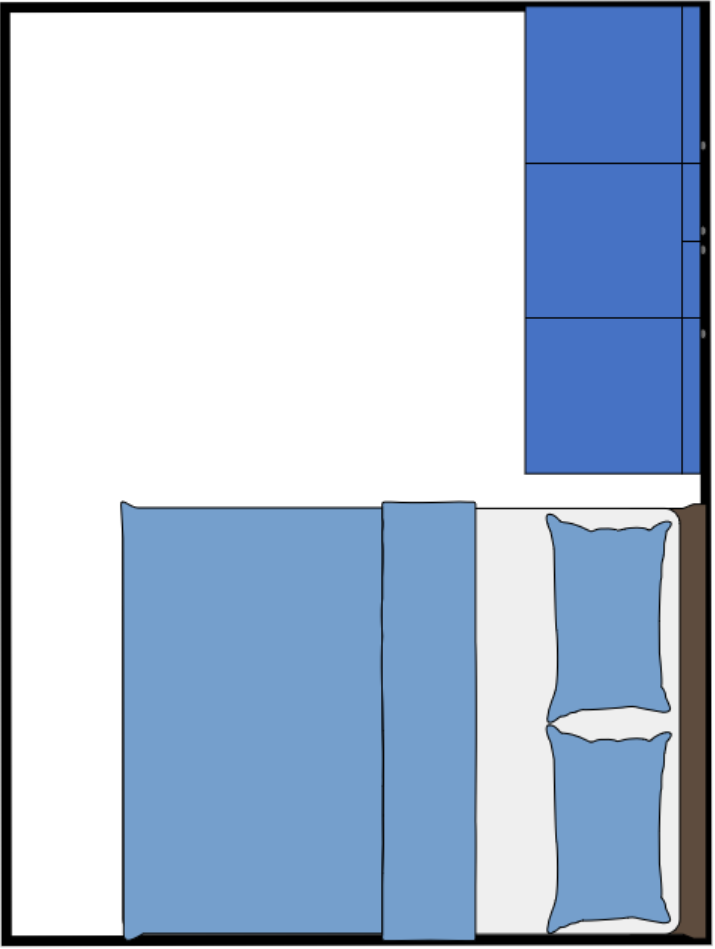
\includegraphics[width=\linewidth]{figures/Liveroom2.png}
        \caption{Bedroom evaluation environment}
        \label{fig:Liveroom2}
    \end{subfigure}
    \hfill
    \begin{subfigure}{0.45\textwidth}
        \centering
        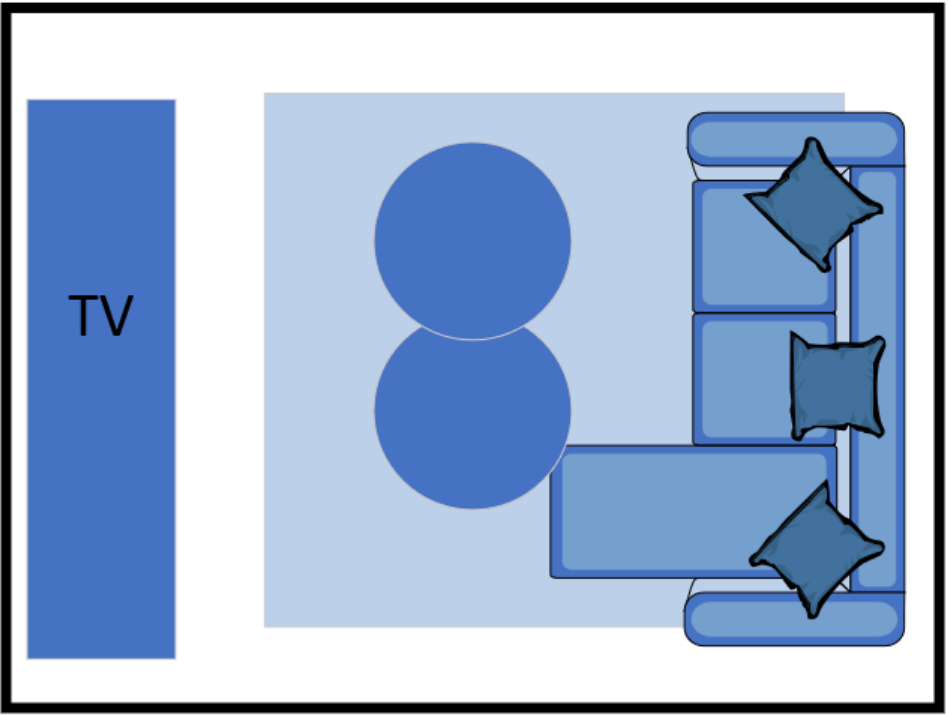
\includegraphics[width=\linewidth]{figures/Liveroom3.png}
        \caption{Living room evaluation environment}
        \label{fig:Liveroom3}
    \end{subfigure}
    
    \caption{Evaluation environments}
    \label{fig:Liveroom}
\end{figure}

For each of the evaluation environments, there was connected an additional IoT device to the same SSID as the Irobot Roomba. These devices generated traffic, simulating a real life smart home environment. the additional IoT devices are list below.

\begin{itemize}
    \item Evaluation environment 1: IPad connected
    \item Evaluation environment 2: Laptop connected
    \item Evaluation environment 3: Smart phone connected
\end{itemize}

\subsubsection{Evaluation Capturing}

All event was triggered once in each of the evaluation environments. Each event had a a 30 minute time window, were the event was triggered and finished within. The overall testing schedule is presented in the list below, were XX is the starting hour. 

\begin{itemize}
    \item Event 1: between XX:00 and XX:30
    \item Event 2: between XX:30 and XX+1:00
    \item Event 3: between XX+1:00 and XX+1:30
    \item Event 4: between XX+1:30 and XX+2:00
    \item Event 5: between XX+2:00 and XX+2:30
    \item Event 6: between XX+2:30 and XX+3:00
\end{itemize}

The event triggering order was decided by a python script, using the library \textit{random}. Scirpt logic presented in Figure \ref{fig:Sudo_code_for_event_order_randomize}. This function was executed three times, ensuring that the order of events was random and had minimum influence cross events.

\begin{figure}[H]
    \centering
    \caption{Sudo code for event order randomize}
    \label{fig:Sudo_code_for_event_order_randomize}
    \begin{lstlisting}[numbers=left]
         event_list = [scheduled_cleaning, Automated_cleaning, Application_triggered_cleaning, Application_start, Physical_triggered_cleaning, Bin_remove]
         for three rounds do:
              shuffle event_list
              print shuffeled list
    \end{lstlisting}
\end{figure}

\subsubsection{Evaluation Data Processing and Filtering}
Data processing and filtering processes are adopted from Chapter \ref{cap:Method}. Because of the added IoT devices, one additional processing step needed to be performed. To filter only based on the corresponding Irobot cloud service we needed to identify the DNS response for \textit{a2uowfjvhio0fa.iot.us-east-1.amazonaws.com}. This request occur once a day, and after a restart of the vacuum cleaner. The capturing was therefore started hour XX - 30 minutes, and the robot vacuum cleaner restarted at hour XX - 20 minutes.

Logic in Figure \ref{fig:Sudo_code_for_IP_extraction_from_DNS_response} was used to extract all IP addresses for \textit{a2uowfjvhio0fa.iot.us-east-1.amazonaws.com} in the DNS response. These addresses was added to the base filter of the extracted event files. All DNS traffic was also included in the base filter, due to their function in the detection algorithm.

\begin{figure}[H]
    \centering
    \caption{Sudo code for IP extraction from DNS response}
    \label{fig:Sudo_code_for_IP_extraction_from_DNS_response}
    \begin{lstlisting}[numbers=left]
        Fuction find_dns_response(even_capture)
          if a2uowfjvhio0fa.iot.us-east-1.amazonaws.com in event_capture
              filter = Responded Ip-addresses and dns
    \end{lstlisting}
 \end{figure}   
 
Evaluation base filter was adopted from Chapter \ref{cap:AnalysisandResults}, this filter exclude tcp-keepalive traffic, NTP, ARP, DHCP and DNS requests for TP-Link online discovery. The evaluation base filter also added two new aspects, they are listed below: 

\begin{itemize}
    \item IP-addresses equal to IP-addresses in the DNS response from \textit{a2uowfjvhio0fa.iot.us-east-1.amazonaws.com}. This excluded all traffic generated by the additional IoT device. Drawback from this implementation was that all traffic towards \textit{50315.ingest.sentry.io} and \textit{s3.amazoneaws.com} was excluded as well. The detection algorithm does not use these tcp sessions for detection, only the DNS packets. It had therefore on impact on the actual detection. 
    \item Capture file duration was 30 minutes, regardless of when the event was triggered or finished. This made the capturing files appear more as a continuous capture, and are not depend on knowledge about when the event was triggered. 
\end{itemize}

\subsection{Evaluation Results}

This subsection is presenting the data processing and rule detection results. First the event triggering sequence, followed by the DNS response IP extraction, then the base filter is presented and finished by the results for event detection. 

\subsubsection{Evaluation Event Triggering Results}
Results from the randomize event order function, are presented in Table \ref{tab:evaleventoverview}. The randomization of the event triggering order, mitigates the influence cross events. 

\begin{table}[H]
\small
\centering
\caption{Evaluation environments event triggering order}
\label{tab:evaleventoverview}
\begin{tabular}{|l|l|l|l|}
\hline
\textbf{Order} & \textbf{Evaluation 1}          & \textbf{Evaluation 2}          & \textbf{Evaluation 3}          \\ \hline
\textbf{1}        & Automated clean                & Application start              & Remove bin                     \\ \hline
\textbf{2}        & App triggered clean            & Scheduled cleaning             & App triggered clean            \\ \hline
\textbf{3}        & Scheduled cleaning             & App triggered clean            & Phy triggered clean            \\ \hline
\textbf{4}        & Phy triggered clean            & Phy triggered clean            & Application start              \\ \hline
\textbf{5}        & Application start              & Automated clean                & Scheduled cleaning             \\ \hline
\textbf{6}        & Bin remove                     & Bin remove                     & Automated cleaning             \\ \hline
\end{tabular}
\end{table}

\subsubsection{DNS response extraction}
All capture files, got processed by the DNS extraction algorithm. DNS responses for \textit{a2uowfjvhio0fa.iot.us-east-1.amazonaws.com}, were found in all of the environments. The extracted IP-addresses are shown in Figure \ref{fig:Evaluation_DNSExtraction}

\begin{figure}[H]
    \centering
    \begin{subfigure}{0.80\textwidth}
        \centering
        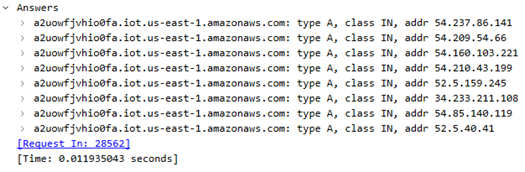
\includegraphics[width=\linewidth]{figures/Evaluation_dns_extraction 1.png}
        \caption{Guestroom DNS extraction}
        \label{fig:Evaluation_DNSextraction_1}
    \end{subfigure}
    \hfill
    \begin{subfigure}{0.80\textwidth}
        \centering
        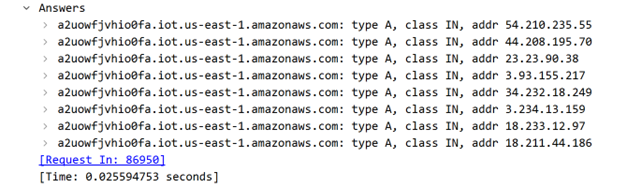
\includegraphics[width=\linewidth]{figures/Evaluation_dns_extraction 2.png}
        \caption{Bedroom DNS extraction}
        \label{fig:Evaluation_DNSextraction_2}
    \end{subfigure}
    \hfill
    \begin{subfigure}{0.80\textwidth}
        \centering
        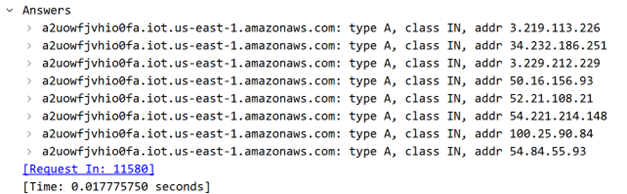
\includegraphics[width=\linewidth]{figures/Evaluation_dns_extraction 3.png}
        \caption{Living room DNS extraction}
        \label{fig:Evaluation_DNSextraction_3}
    \end{subfigure}
    \caption{Evaluation environment DNS extraction}
    \label{fig:Evaluation_DNSExtraction}
\end{figure}

\subsubsection{Evaluation base filter}
 DNS responses included several IP-addresses for the corresponding Irobot cloud service, this is used by Irobot to load balance the traffic towards their services \cite{dns_load_balancing}.The Irobot Roomba then only established a connection to one of the IP addresses. A TCP handshake towards one of the IP in the DNS response was identified right after the DNS response in Wireshark. The identification of these are presented in Figure \ref{fig:evaluation_corresponding_cloud}. This is a easy way for any attacker to identify corresponding traffic based on DNS requests. The used base filters are listed below, and are identical for all environments except the corresponding Irobot hosts. 

\begin{itemize}
    \item Evaluation filter: \begin{itemize}
                                \item ((frame.time >= "Apr <day>, 2023 XX:00:00") \&\& (frame.time <= "Apr <day>, 2023 XX:30:00")) AND
                                \item (frame.len > 97) AND 
                                \item  ((ip.addr == <DNS response IP>) or (dns \&\& ip.dst == 192.168.0.56))
                            \end{itemize}
    \item DNS response IP:  \begin{itemize}
                                \item Guestroom: 54.237.86.141 
                                \item Bedroom: 3.93.155.217 
                                \item Living room: 3.219.113.226 
                            \end{itemize}
\end{itemize}

\begin{figure}[H]
    \centering
    
    \begin{subfigure}{0.80\textwidth}
        \centering
        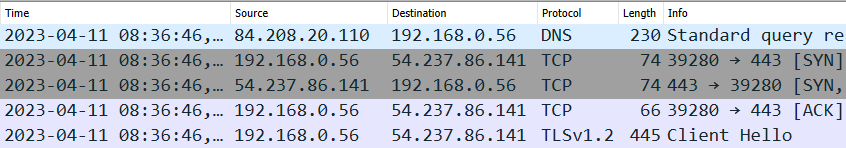
\includegraphics[width=\linewidth]{figures/Evaluation_cloud_detection1.png}
        \caption{Guestroom corresponding could detection}
        \label{fig:Evaluation_coulddetection_1}
    \end{subfigure}
    \hfill
    \begin{subfigure}{0.80\textwidth}
        \centering
        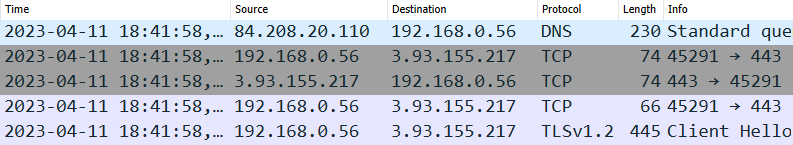
\includegraphics[width=\linewidth]{figures/Evaluation_cloud_detection2.png}
        \caption{Bedroom corresponding could detection}
        \label{fig:Evaluation_clouddetection_2}
    \end{subfigure}
    \hfill
    \begin{subfigure}{0.80\textwidth}
        \centering
        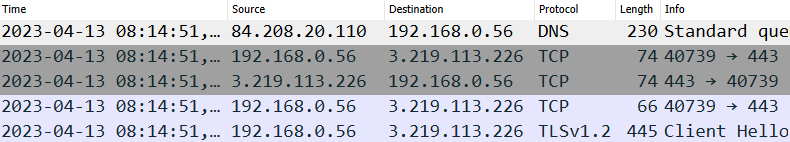
\includegraphics[width=\linewidth]{figures/Evaluation_cloud_detection3.png}
        \caption{Living room corresponding could detection}
        \label{fig:Evaluation_clouddetection_3}
    \end{subfigure}
    
    \caption{Evaluation environments corresponding could detection}
    \label{fig:evaluation_corresponding_cloud}
\end{figure}

\subsubsection{Evaluation Detection Results}
All 18 filtered event capturing files was processed by the detection algorithm in Appendix \ref{app:DetectionAlgorithm}. No manual analysis was done to the files before hand. Detection results are presented in Table \ref{tab:Evaluation results}. Scheduled cleaning and Physical triggered cleaning is merged to (Sch \& Phy). This because they could not be separated in Chapter \ref{cap:AnalysisandResults}.

\begin{table}[H]
\small
\centering
\caption{Evaluation results}
\label{tab:Evaluation results}
\begin{tabular}{|c|c|c|c|c|c|}
\hline
\textbf{Event}        & Auto clean & App clean & Sch \& Phy & App start & Bin removed \\ \hline
\textbf{Success rate} & 100\%           & 100\%             & 100\% & 100\%             & 0\%         \\ \hline
\end{tabular}
\end{table}

The rules and detection algorithm was able to detect all events with 100\% accuracy, except bin remove. Cleaning detection resulted is True positive for all the cleaning event. If a cleaning event was detected, but not automated cleaning or application start packet sequence, it was categorized as either scheduled or physical triggered cleaning. To differentiate these two events there should be implemented a time detection of the first "cleaning packet sequence". This timestamp can determine if it is most likely a scheduled or a physical triggered cleaning. 

Bin remove detection gave False negative for all the bin remove events. This might be because the ejection of the bin was executed without causing the Irobot Roomba to lose connection to the charging connectors. The detection algorithm also had False positive identification of bin remove event for 66\% of the automated cleaning event. The bin remove signature is therefore not usable in detection of bin removal. 


\section{Our Answer to Research Question 1}
\textbf{Which private information can be gathered from robot vacuum cleaner by carrying out a passive sniffing attack in a smart environment?}

It is possible to identify the presence of an Irobot vacuum cleaner inside a smart environment based on the WLAN or LAN capture itself. In WLAN eavesdropping an attacker can lookup all  MAC addresses against open source registers. For LAN capture the presence of DNS requests to any Irobot owned domain will place a device behind the WAN address.

Other Irobot Roomba i7 events can be detected in a smart environment. Automated cleaning can be triggered by the use of location services, garage openers and door locks. All these automated triggers are indications that users are leaving the smart environment. 

If implementations to differentiate physical triggered and scheduled cleaning are added, the detection of physical triggered cleaning will revile user activity inside the smart environment. Schedule cleaning on the other hand can give away user routines. We can assume that users usually configure scheduled cleaning when there is a high probability that there is no one at the premise. This can revile on site routines. 

For application triggered cleaning and application start it is harder to identify the actual privacy exposure. The identification of these events can revile more information if observed during longer time periods. Then user patterns and behaviors can be exposed. Users could trigger cleaning,  every time they are leaving for work or the gym.

As mentioned for WLAN capturing, an attacker can extract private information as soon as the capturing is started. This because the filter and identification of traffic is based in MAC addresses. For LAN an attacker will have to eavesdropp WAN traffic for maximum of 24 hours before the DNS request to \textit{a2uowfjvhio0fa.iot.us-east-1.amazonaws.com} is sent, and the corresponding Irobot cloud service is identified. 

\section{Our Answer to Research Question  2}
\textbf{How can information exposed by the eavesdropping be misused by an attacker?} 

Private information exposed to an attack can be utilized to identify user behavior and routines. This could potentially revile habits of when the user is leaving the environment, and identify user presence with high confidence. This information can be used to target user environment during empty hours, or address the environment when the user is present. Such information can also be sold to other actors. 

The identification of devices can be used  to target attacks, based on IoT inventory. Spear phishing \cite{spear_phishing} will be more effective. They can also target attack to exploit known or unknown vulnerabilities for the identified devices. This will increase the success rate of an attack. Exposed privacy information will threaten the security of any smart environment. 

\section{Our Answer to Research Question  3}
\textbf{Which security measures can be implemented to limit the exposed data and decrease the risk of misuse?} 

The most efficient way to defend against the detection algorithm, would be to implement a traffic sharper. This device could disrupt the predicted network traffic flows, pad existing packets or inject packets to break the patters. This will be an effective way to defend against this in LAN or WLAN eavesdropping. A disadvantage with traffic shaping, will be higher latency, more data processing on local equipment. Implementation of traffic shaper could be on the robot vacuum cleaner itself, this would secure the communication regardless of the smart home environment infrastructure. Or as a service within the smart environment, then the overall security of the smart environment would increase. 

Irobot could implement random MAc addressing \cite{random_mac_bernardos2020rfc} for WLAN communication. This would allow the Irobot vacuum cleaner to use a random MAC address each time is connects to a new network, or change randomly to mislead an attacker. 

As for WAN or LAN tarffic, DNS is an easy identifier. The initial session needs to be established based on a DNS request, but consecutive changes could be transferred through the encrypted communication channel established. This could mitigate the use of DNS as detection. 




\chapter{Discussion}
This chapter discusses the challenges, processes and decisions throughout the research. The main topics is the thesis' answer to the research questions. Further, the limitation of Wi-Fi scope, how the events were triggered, why human analysis was selected and the reason to exclude the complexity of eavesdropping. 

\section{Collection of Wi-Fi Traffic}
The selected TP-Link AP had Internet Group Management Protocol (IGMP) \cite{igmp_rfc2236} default enabled. This protocol enables devices on a local network to subscribe to different multicast groups. Return traffic will then be addressed to the multicast group and not the device's MAC address. Due to this functionality, only the outbound traffic generated form the robot vacuum cleaner was captured during the standby event. Initial analysis of the standby traffic verified this when WLAN base filter was applied. These findings are shown in Figure \ref{fig:WLANIGMP_enabled}.

\begin{figure}[H]
    \centering
    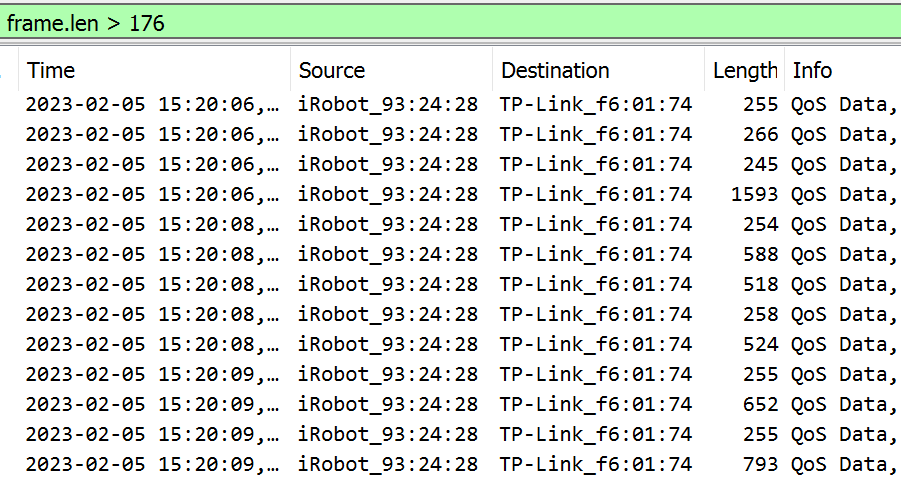
\includegraphics[width=0.8\textwidth]{figures/WLAN_IGMP_enabled.png}
    \caption{Wireshark WLAN capture, included base filter and enabled IGMP}
    \label{fig:WLANIGMP_enabled}
\end{figure}

If IGMP enabled Wi-Fi would to be in the scope of this thesis, a process of filtering based on multicast group addresses should have been implemented. A 20 minutes \textit{Application triggered cleaning} capturing was conducted in \textbf{Oslo} capturing only traffic including the MAC address of the AP. The capture included 9,342 packets, which is 340\% more than LAN traffic average for the same event. By applying a Wireshark filter, excluding all traffic except Irobot and multicast MAC addressed, we identified the new IGMP traffic flow. This is shown in Figure \ref{fig:WLANIGMP_all_enabled}. 

\begin{figure}[H]
    \centering
    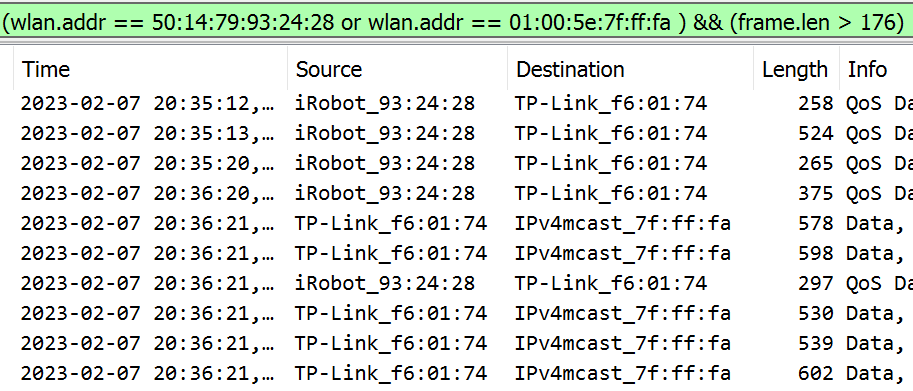
\includegraphics[width=\textwidth]{figures/WLAN_IGMP_ALL.png}
    \caption{WLAN IGMP application triggered cleaning test in Oslo}
    \label{fig:WLANIGMP_all_enabled}
\end{figure}

This increases the complexity of the filtering mechanisms and identification of multicast traffic would be possible in \textbf{Oslo} and \textbf{Drammen}. The complexity occurs when more then one IoT device is connected to the same network. Devices can subscribe to the same or a new multicast group making the wireless environment more complex and hard to navigate in. IGMP is not used in all Wi-Fi networks \cite{wifi_ieee80211} and it is therefor disabled on the AP. 

\section{Event Triggering}
As shown in Chapter \ref{cap:AnalysisandResults}, several events were triggered during the same day and with limited time period between them. The reason for this is the time constraint of this master project and the availability of smart environments. This increases the possibility of cross event influence, especially in the end of cleaning when the Irobot Roomba uploads cleaning data to the cloud service at \textit{s3.amazonsaws.com}. To mitigate the influence, it was decided to only focus on the event initiation and not the end of cleaning reporting. Event triggering traffic is assumed to be the same regardless of previous events. 

Real-life simulation of a smart environment is hard to recreate as there will not be triggered 5 cleaning events, within 2 hours. Event triggering timestamps in this project will appear unrealistic due to structured triggering in a short time period. Timestamps captured and identified in this research can therefore not be used in attributing events, but as mentioned in the analysis it could be a good attribute to include in the analysis and extraction of user private information.  

\section{Method of Analysis}
Both human-based analysis and machine learning were discussed as the traffic analysis method in this project. Several other researches have used machine learning to extract information from network traffic based on various attributes. During the literature review no documentation describing Irobot Roomba's communication pattern or protocols was found, Irobot did also not reply with information upon requests for this information. Either way, the data would have to be pre-processed by a human to identify which attributes that could be used in further analysis. The analysis method was therefore decided to be manual human-learn rule-based. 

\section{The Complexity of Eavesdropping}
The level of complexity of conducting an eavesdropping attack for WLAN, LAN or WAN is not addressed in this thesis. This is a topic which should be addressed in separate research, due to the variety of devices and configurations in different smart environments. Smart environments used in this project only serve Internet access to exclude possible local configuration. 

In wireless eavesdropping, an attacker would only need to be in wireless range of the targeted devices to collect corresponding network traffic. Eavesdropping devices can be placed in the vicinity of the smart environment or installed inside an environment, collected data can be stored locally or exported to a online service through Internet connection. There are pros and cons with the different approaches which is not addressed. For LAN and WAN eavesdropping the attacker would need physical access to the local network, or exploit remote access to network devices. These operations challenge both physical and technical security and are therefore out of scope for this thesis. 

\section{Our Answer to Research Question 1}
\textbf{Which private information can be gathered from a robot vacuum cleaner by carrying out a passive sniffing attack in a smart environment?}

It is possible to identify the presence of an Irobot Roomba i7 vacuum cleaner inside a smart environment based on the WLAN or LAN capture itself. In WLAN, an attacker can eavesdrop and lookup all  MAC addresses against open source registers. For LAN capture the presence of DNS requests to any Irobot owned domain will place a device behind the WAN address.

The signature detection algorithm proposed and evaluated in this project was able to identify and attribute different events conducted on the Irobot Roomba i7. Detection of \textit{Automated cleaning} exposed information of when the user left the location, revealing private information. By observing the last five \textit{Automated cleaning} events in \textbf{Oslo} is was possible to identify when the user left work, collecting an analysis of event triggering over a longer time period can expose user behaviour. \textit{Application triggered cleaning} and \textit{Application start} was also identified exposing user interaction with the Irobot Roomba.

If implementations to differentiate physical triggered and scheduled cleaning are added, the detection of physical triggered cleaning will reveal user activity inside the smart environment. Schedule cleaning on the other hand can give away user routines. We can assume that users usually configure scheduled cleaning when there is a high probability that there is no one at the location. This can reveal on site routines. 

For application triggered cleaning and application start it is harder to identify the actual privacy exposure. The identification of these events can reveal more information if observed during longer time periods. Then user patterns and behaviors can be exposed. Users could trigger cleaning every time they are leaving for work or the gym.

As mentioned for WLAN capturing, an attacker can extract private information as soon as the capturing is started because identification of the traffic is based in MAC addresses. For LAN, an attacker will have to eavesdrop WAN traffic for maximum of 24 hours before the DNS request to \textit{a2uowfjvhio0fa.iot.us-east-1.amazonaws.com} is sent, and the corresponding Irobot cloud service is identified. 

\section{Our Answer to Research Question  2}
\textbf{How can information exposed by the eavesdropping be misused by an attacker?} 

Private information exposed in an attack can be utilized to identify user behavior and routines. This could potentially reveal habits of when the user is leaving the environment, and identify user presence with high confidence. This information can be used to target user environment during empty hours, or address the environment when the user is present. Such information can also be sold to other actors. 

The identification of devices can be used  to target attacks, based on IoT inventory. Spear phishing \cite{spear_phishing} will be more effective. They can also target attacks to exploit known or unknown vulnerabilities for the identified devices. This will increase the success rate of an attack. Exposed privacy information will threaten the security of any smart environment. 

\section{Our Answer to Research Question  3}
\textbf{Which security measures can be implemented to limit the exposed data and decrease the risk of misuse?} 

The most efficient way to defend against the detection algorithm, would be to implement traffic shaping. This device could disrupt the predicted network traffic flows, pad existing packets or inject packets to break the patterns. This will be an effective way to defend against this in LAN or WLAN eavesdropping. A disadvantage with traffic shaping, will be higher latency and more data processing on local equipment. Implementation of traffic shaping could be on the robot vacuum cleaner itself, this would secure the communication regardless of the smart home environment infrastructure. Another approach is to implement this as a service within the smart environment, then the overall security of the smart environment would increase. 

Irobot should implement random MAC addressing \cite{random_mac_bernardos2020rfc} for WLAN communication. This would allow the Irobot vacuum cleaner to use a random MAC address each time is connects to a new network, or change randomly to mislead an attacker. 

As for WAN or LAN traffic, DNS is an easy identifier due to the use of Wi-Fi channel encryption. The initial session needs to be established based on a DNS request revealing the the IP address to the initial corresponding host. However, the daily change of corresponding host could be communicated through the secure connection hiding the change in cloud server host. This would make the detection of Irobot Roomba traffic harder to conduct by an attacker.


\chapter{Conclusions}
In this thesis, we have proposed event detection algorithms to perform event detection and attribution, of an Irobot Roomba i7 robot vacuum cleaner. Data collection was done in two different smart home environments, where the same robot vacuum cleaner was deployed. A baseline traffic capture was conducted over a time period of 14 days, this capture was used to identify all event irrelevant traffic. Based on these finding all IP-packets less then 98 bytes was excluded for further analysis.  

The result was a reduction of more then 99\% of the captured traffic. The same base-filter was applied to the event capturing files, leaving only the traffic relevant to the actual events. IP-addresees, DNS responses and TCP packet length sequences was analyzed. The findings resulted in event specific signatures and a detection algorithm. Five different signatures was proposed. 

To evaluate the proposed event detection algorithm, we deployed the Irobot Roomba i7 in three new smart home environments. Each of the environments had other IoT devices connected to create a more representable smart home. The detection algorithms detected 4 out of 5 with 100\% accuracy. The last event \textit{Bin Remove} gave False negative in all three evaluation environments.

This thesis' results can with high confidence identify and attribute different events triggered on an Irobot Roomba i7, based on WAN network traffic. This will expose user routines and habits. It is also identified the same type of packet sequence in WLAN, which makes the detection transferable to wi-fi as well. Security measures should therefore be used by the Robot vaccum cleaner vendors ti mitigate the risk of these eavesdropping attacks. 

\section{Future work}
Future research should look into development of an automated tool, which can capture, process and analysis network traffic automatically. This would ease the process, and enable researches to extract similar results from a series of robot vacuum cleaners. Future it could compare different vendors and, evaluate privacy differences cross vendors. This would contribute to better security awareness and design for all users of robot vacuum cleaners. 

Another diction of research would be to look into irobot integration. Create real life smart environments, where devices that can integrate and trigger vacuum cleaner events is deployed. Device attribution and traffic correlation, could expose even more private information about users.   








\chapter*{\bibname}
\printbibliography[heading=none]

%\input{chapters/papers.tex}

\appendix
\appendixpage
\chapter{Detection Algorithm}
\label{app:DetectionAlgorithm}

\begin{lstlisting}[numbers=left]
# Python code, Signeture detection
import pyshark
from pyshark.packet import consts
from pyshark.packet.common import Pickleable
import matplotlib
import numpy
import os


def cleaning_conf(c_conf):
    
    dns_o_i_s_i = False
    dns_aws = False
    clean_end = None
    
    #Loop all packets in capture
    for packet in cap:

        #find DNS response lager then 100 bytes 
        if packet.highest_layer == 'DNS' and packet.ip.dst_host == wan_addr:
            #print('dns')
            #find cleaning dns response
            if packet.dns.resp_name == 'o550315.ingest.sentry.io':
                dns_o_i_s_i = True
                #print('dns1')
            if packet.dns.resp_name == 's3.amazonaws.com':
                dns_aws = True
                #print('dns2')
    
        if dns_o_i_s_i and dns_aws == True:
            c_conf =+ 10
            return c_conf

    return c_conf

def get_type_of_cleaning():
    indication_sc = 0
    indication_tc = 0
    cleaning_type = None
    clean_start = None

    #Loop through all packets in capture
    for packet in cap:
        #Add indication for sc
        if  packet.ip.dst_host == '192.168.0.56' and packet.length == ('1101' or '1107'):
            indication_sc = indication_sc + 1
            
        #Add indication for tc
        if packet.ip.dst_host == '192.168.0.56' and packet.length == ('1105' or '1106' or '1099'):
            indication_tc = indication_tc + 1

    if indication_sc > indication_tc:
        cleaning_type = 'scheduled cleaning'
    if indication_sc < indication_tc:
        cleaning_type = 'triggered cleaning'
    

    return cleaning_type

def open_application_conf(oa_conf):
    #open application True/False
    open_application = False
    ao_time = 'Opening time not identified'
    oa_initiator = [209, 289, 316]
    oa_initiator_1 = [209, 315, 289]
    for packet in cap:
        if packet.length == '209':
            ao_time = packet.sniff_time
            #print(ao_time)
    
        if 209 in packet_length[0:20]:
            oa_index = packet_length_dst.index(209)
            oa_start_compare = packet_length_dst[oa_index:oa_index + len(oa_initiator)]
            open_application = numpy.allclose(oa_initiator, oa_start_compare, atol= 3)
            open_application_1 = numpy.allclose(oa_initiator_1, oa_start_compare, atol= 3)
            if (open_application or open_application_1) == True:
                oa_conf =+ 10
                return oa_conf

        if 208 in packet_length[0:20]:
            oa_index = packet_length_dst.index(208)
            oa_start_compare = packet_length_dst[oa_index:oa_index + len(oa_initiator)]
            open_application = numpy.allclose(oa_initiator, oa_start_compare, atol= 3)
            open_application_1 = numpy.allclose(oa_initiator_1, oa_start_compare, atol= 3)
            if (open_application or open_application_1) == True:
                oa_conf =+ 10
                return oa_conf

        if 207 in packet_length[0:20]:
            oa_index = packet_length_dst.index(207)
            oa_start_compare = packet_length_dst[oa_index:oa_index + len(oa_initiator)]
            open_application = numpy.allclose(oa_initiator, oa_start_compare, atol= 3)
            open_application_1 = numpy.allclose(oa_initiator_1, oa_start_compare, atol= 3)
            if (open_application or open_application_1) == True:
                oa_conf =+ 10
                return oa_conf

    
    
    return oa_conf

def find_packet_seq(tc_confident):
    triggered_cleaning = [503, 175, 509, 1106, 179, 439, 1099, 179, 445, 1105, 176]
    scheduled_cleaning = [179, 447, 1107, 176, 476, 176, 617, 179, 253, 626, 179, 447, 1107]
    oopen_application = [209, 289, 316, 176, 187, 409]
    bin_entered = [179, 186, 410]
    auto_clean = [316, 289, 176, 187, 409]
    
    if 503 in packet_length:
        tc_index = packet_length.index(503)
        tc_compare = packet_length[tc_index:tc_index + len(triggered_cleaning) ]
        tc_test = numpy.allclose(triggered_cleaning, tc_compare, atol= 1)

        if tc_test == True:
            tc_confident = tc_confident + 10

    return tc_confident

def auto_clean_conf(ac_conf, packet_length):
    auto_clean = [316, 289, 176, 187, 409]
    auto_clean_1 = [289, 316, 176, 187, 409]

    if 207 in packet_length[0:30]:
        return ac_conf
    if 208 in packet_length[0:30]:
        return ac_conf
    if 209 in packet_length[0:30]:
        return ac_conf


    if 316 in packet_length:
        ac_index = packet_length.index(316)
        ac_start_compare = packet_length[ac_index:ac_index + len(auto_clean)]
        ac_indication = numpy.allclose(auto_clean, ac_start_compare, atol= 1)
        if ac_indication == True:
            ac_conf =+ 10
            return ac_conf
    
    if 315 in packet_length:
        ac_index = packet_length.index(315)
        ac_start_compare = packet_length[ac_index:ac_index + len(auto_clean)]
        ac_indication = numpy.allclose(auto_clean, ac_start_compare, atol= 1)
        if ac_indication == True:
            ac_conf =+ 11
            return ac_conf

    if 288 in packet_length:
        ac_index = packet_length.index(288)
        ac_start_compare = packet_length[ac_index:ac_index + len(auto_clean_1)]
        ac_indication = numpy.allclose(auto_clean_1, ac_start_compare, atol= 1)
        if ac_indication == True:
            ac_conf =+ 12
            return ac_conf
        
    if 289 in packet_length:
        ac_index = packet_length.index(289)
        ac_start_compare = packet_length[ac_index:ac_index + len(auto_clean_1)]
        ac_indication = numpy.allclose(auto_clean_1, ac_start_compare, atol= 1)
        if ac_indication == True:
            ac_conf =+ 13
            return ac_conf
            
    return ac_conf   

def trigger_clean_conf(tc_conf, oa_conf, c_conf):
    
    #If there is a cleaning and tha application is opened, we can say that it is likely that is has been a triggered clean
    if oa_conf and c_conf == 10:
        tc_conf =+ 10


    return tc_conf

def physical_cleaning_conf(pc_conf, packet_length_src):
    physical_clean = [176, 173, 179, 443, 177]
    physical_clean_1 = [176, 443, 179, 443, 177]
    count = 0
    #The value can be 172, 176, 175 and 179
    for packet in packet_length_src:
        
        if 172 <= packet <= 179:
          pc_compare = packet_length_src[count:count + len(physical_clean)]
          pc_indicator = numpy.allclose(physical_clean, pc_compare, atol= 15)
          pc_indicator_1 = numpy.allclose(physical_clean_1, pc_compare, atol= 5)

          if pc_indicator == True:
              pc_conf =+ 10
              return pc_conf
          
          if pc_indicator_1 == True:
              pc_conf =+ 11
              return pc_conf
        
        count = count + 1
    

    return pc_conf

def remove_bin(br_conf):

    removebin_value = '410'
    for packet in cap:
        if packet.length ==  '410':
            return 10
        if packet.length == "411":
            return 10
    return 0

def dns_cleaning(c_conf, dns_names):
    
    if 'o550315.ingest.sentry.io' and 's3.amazonaws.com' in dns_names:
        return 10
    else:
        return 0

# MAIN Function is starts


folder = [r'C:\Users\benja\Documents\Mater test results\LAN\Live\Env3_dns']
files = os.listdir(folder[0])
#print(folder[0] + '\\' + files[0])
wan_addr = '192.168.0.56'

for file in files:
    ac_conf = 0
    oa_conf = 0
    sc_conf = 0
    tc_conf = 0
    rb_conf = 0
    pc_conf = 0
    c_conf = 0
    

    file_path = str(folder[0] + '\\' + file)
    cap = pyshark.FileCapture(file_path)
    cap.load_packets()
    packet_length = [2000]
    packet_length_dst = [2000]
    packet_length_src = [2000]
    packet_time = []
    dns_names = []
    


    for packet in cap:
        if packet.highest_layer != 'DNS':

            if int(packet.length) != packet_length[-1]:
                packet_length.append(int(packet.length))
                #packet_time.append(int(packet.sniff_time))

                if packet.ip.dst_host == wan_addr:
                    packet_length_dst.append(int(packet.length))

                if packet.ip.src_host == wan_addr:
                    packet_length_src.append(int(packet.length))
        else:
            dns_names.append(packet.dns.resp_name)
    

                

    print(file)
    #print(packet_length_dst)
    ac_conf =+ auto_clean_conf(ac_conf, packet_length)
    oa_conf =+ open_application_conf(oa_conf)
    #c_conf =+ cleaning_conf(c_conf)
    c_conf =+ dns_cleaning(c_conf, dns_names)
    tc_conf =+ trigger_clean_conf(tc_conf, oa_conf, c_conf)
    #pc_conf =+ physical_cleaning_conf(pc_conf, packet_length_src)
    rb_conf =+ remove_bin(rb_conf)
    #print(packet_length_dst[0:20])
    #print(dns_names)

    #print("Auto clean  " + str(ac_conf) + '  Open application  '+ str(oa_conf) + '   Cleaning  ' + str(c_conf) + '  triggered  ' + str(tc_conf) + '  Pysical  ' + str(pc_conf))
    if ac_conf > 0:
        print('Auto Clean')
    if tc_conf > 0:
        print('Triggered Cleaning')
    if c_conf > 0 and ac_conf == 0 and tc_conf == 0:
        print('Scheduled or Physical cleaning')
    if rb_conf > 0:
        print('Bin is removed')
    if oa_conf > 0 and tc_conf == 0:
        print('application is opened')

    
    


    




\end{lstlisting}
\chapter{Packet Lengths Extraction Algorithm}
\label{app:Packetlengthex}


\begin{lstlisting}[numbers=left]
     import pyshark
from pyshark.packet import consts
from pyshark.packet.common import Pickleable
import matplotlib
import numpy
import os

folder = [r'filepath']
files = os.listdir(folder[0])
#print(folder[0] + '\\' + files[0])
sum_lenght=  []
sum_nr = []
print(files)
for file in files:

    file_path = str(folder[0] + '\\' + file)
    #print(file)
    cap = pyshark.FileCapture(file_path)
    cap.load_packets()
    packet_lengths = []
    packet_count = 0
    
    

    for packet in cap:
        
       # if packet.ip.dst_host == '192.168.0.56':
       #     packet_lengths.append('D ' + packet.length)
       # else:
       #     packet_lengths.append('S ' + packet.length)
        packet_lengths.append(int(packet.length))
        packet_count = packet_count + 1


    print(file)
    print(packet_count)
    print(sum(packet_lengths))
    sum_lenght.append(sum(packet_lengths))
    sum_nr.append(packet_count)
    #if len(packet_lengths) >= 20:
    #    print(packet_lengths[0:20])
    #else:
    #    print(packet_lengths[0:len(packet_lengths)])


print(sum(sum_lenght)/10)   
print(sum(sum_nr)/10)
print(sum_lenght)   
print(sum_nr)    
    \end{lstlisting}
\chapter{DNS Extraction Algorithm}
\label{app:DNSex}


\begin{lstlisting}[numbers=left]
import pyshark
import os


def dns_ip_find ():
    
    
    #Loop all packets in capture
    for packet in cap:

        #find DNS response lager then 100 bytes 
        if packet.highest_layer == 'DNS' and packet.ip.dst_host == '192.168.0.56':
            #print('dns')
            #find cleaning dns response
            if packet.dns.resp_name == 'a2uowfjvhio0fa.iot.us-east-1.amazonaws.com':
                print(packet.dns.pretty_print())
                print(packet.sniff_time)
                print(packet.number)
                print('dns1')

            if packet.dns.resp_name == 'unauth1.prod.iot.irobotapi.com':
                print(packet.dns.pretty_print())
                print(packet.sniff_time)
                print('dns1')

            if packet.dns.resp_name == 'disc-prod.iot.irobotapi.com':
                print(packet.dns.pretty_print())
                print(packet.sniff_time)
                print('dns1')


            if packet.dns.resp_name == '0.irobot.pool.ntp.org':
                print(packet.dns.pretty_print())
                print(packet.sniff_time)
                print('dns1')
            if packet.dns.resp_name == 'o550315.ingest.sentry.io':
                print(packet.number)
            
    
 

    return None


folder = [r'C:\Users\benja\Documents\Mater test results\LAN\Live\Env1_dns']
files = os.listdir(folder[0])

for file in files:

    print(file)
    file_path = str(folder[0] + '\\' + file)
    cap = pyshark.FileCapture(file_path, display_filter='dns')
    cap.load_packets()

    dns_ip_find()
\end{lstlisting}

\end{document}

